\documentclass{article}

\usepackage[colorlinks=true, allcolors=blue]{hyperref}
\usepackage[letterpaper,top=2cm,bottom=2cm,left=3cm,right=3cm,marginparwidth=1.75cm]{geometry}
\usepackage[T1]{fontenc}
\usepackage[bottom]{footmisc} %paczka do poprawnego pozycjonowania obiektów \footnote
\usepackage{xcolor} %paczka do ustawiania koloru tekstu
\usepackage{listings} %paczka do tworzenia własnego stylu kodu
\usepackage[polish]{babel}
\usepackage[utf8]{inputenc}
\usepackage{amsmath}
\usepackage{autobreak}
\usepackage{graphicx}
\usepackage{caption}
\usepackage{tabularx}
\usepackage{pifont}
\usepackage{svg} %paczka do wyświetlania obrazów w formacie svg
\usepackage{wrapfig} %paczka do zawijania tekstu wokół figur
\usepackage[nottoc,numbib]{tocbibind} %dodaje dział "Literatura" do spisu treści
\usepackage{moresize} %paczka dodająca większą ilość rozmiarów czonki

\usepackage{url} % package to format url
\makeatletter
\g@addto@macro{\UrlBreaks}{\UrlOrds} % dodanie "-" do znaków przełamujących adresy url
\makeatother

\hypersetup{linkcolor=black, citecolor={black}, urlcolor={black}} %zmiana koloru linków

\definecolor{comment}{RGB}{50, 133, 96}
\definecolor{brackets}{RGB}{0, 117, 212}
\definecolor{type}{RGB}{191, 130, 65}
\definecolor{purple}{RGB}{125, 77, 158}
\definecolor{background}{HTML}{EEEEEE}

\lstdefinelanguage{jsonSchema}{
    basicstyle=\normalfont\ttfamily,
    numbers=left,
    numberstyle=\scriptsize,
    stepnumber=1,
    numbersep=8pt,
    showstringspaces=false,
    breaklines=true,
    frame=lines,
    backgroundcolor=\color{background},
    literate=
     *{str}{{{\color{type}str}}}{3}
      {int}{{{\color{type}int}}}{3}
      {dict}{{{\color{type}dict}}}{4}
      {float}{{{\color{type}float}}}{5}
      {None}{{{\color{type}None}}}{4}
      {bool}{{{\color{type}bool}}}{4}
      {|}{{{\color{type}|}}}{1}
      {,}{{{\color{type},}}}{1}
      {[}{{{\color{type}{[}}}}{1}
      {]}{{{\color{type}{]}}}}{1}
      {(opcjonalnie)}{{{\color{comment}\textit{(opcjonalnie)}}}}{12}
      {:}{{{\color{brackets}{:}}}}{1}
      {"}{{{\color{brackets}{"}}}}{1}
      {\{}{{{\color{brackets}{\{}}}}{1}
      {\}}{{{\color{brackets}{\}}}}}{1},
}
% fragment kodu aby znaki ")" były kolorowane poprawnie
\usepackage{etoolbox}
\makeatletter

\patchcmd{\lsthk@SelectCharTable}{%
  \lst@ifbreaklines\lst@Def{`)}{\lst@breakProcessOther)}\fi
}{%
}{
}{
}

\makeatother
\lstdefinelanguage{pythonSchema}{
    basicstyle=\normalfont\ttfamily,
    columns=fixed,
    numbers=left,
    numberstyle=\scriptsize,
    stepnumber=1,
    numbersep=8pt,
    showstringspaces=false,
    breaklines=true,
    frame=lines,
    backgroundcolor=\color{background},
    moredelim=*[s][\color{type}]{"}{"}, % wszystko pomiędzy " i " ma mieć kolor
    moredelim=*[s][\color{type}]{'}{'}, % wszystko pomiędzy ' i ' ma mieć kolor
    literate=
     *
      {while}{{{\color{purple}while}}}{4}
      {else}{{{\color{purple}else}}}{4}
      {elif}{{{\color{purple}elif}}}{4}
      {for}{{{\color{purple}for}}}{2}
      {def}{{{\color{purple}def}}}{2}
      {if}{{{\color{purple}if}}}{2}
      {fontTiny}{fontTiny}{7}
      {(}{{{\color{brackets}(}}}{1}
      {)}{{{\color{brackets})}}}{1}
      {[}{{{\color{brackets}{[}}}}{1}
      {]}{{{\color{brackets}{]}}}}{1}
      {\{}{{{\color{brackets}{\{}}}}{1}
      {\}}{{{\color{brackets}{\}}}}}{1}
      {:}{{{\color{brackets}{:}}}}{1}
      {=}{{{\color{brackets}{=}}}}{1}
      {list[Button]}{{{\color{type}list[Button]}}}{10}
      {list[list[pygame.Surface,}{{{\color{type}list[list[pygame.Surface,}}}{20}
      {pygame.font.Font]]}{{{\color{type}pygame.font.Font]]}}}{15}
      {None}{{{\color{type}None}}}{4}
      {->}{{{\color{type}->}}}{2},
}

\begin{document}
\begin{center}
    \begin{LARGE}
        \textbf{UNIWERSYTET GDAŃSKI}
    \end{LARGE}
\end{center}

\begin{center}
    \begin{LARGE}
        \textbf{WYDZIAŁ MATEMATYKI, FIZYKI I INFORMATYKI}
    \end{LARGE}
\end{center}

\vspace{0.5cm}

\begin{center}
    \begin{Large}
        \textbf{Paweł Olszewski}
    \end{Large}
\end{center}

\begin{center}
    \textbf{numer albumu: 274983}
\end{center}

\begin{center}
    \textbf{współautorzy: Kacper Krüger, 274977}\\
    \hspace{3.35cm}\textbf{Maksymilian Keller, 274952}\\
    \hspace{3.45cm}\textbf{Mateusz Maćkowiak, 275006}
\end{center}

\vspace{2cm}

\textit{Kierunek studiów: Informatyka, profil praktyczny}

\vspace{2cm}

\begin{center}
    \begin{LARGE}
        \textbf{Projekt Frostbite}
    \end{LARGE}
\end{center}

\vspace{3cm}

\begin{flushright}
    Praca licencjacka\\wykonana\\pod kierunkiem\\dr inż. Łukasza Kusznera
\end{flushright}

\vspace{6cm}

\begin{center}
    \textbf{Gdańsk 2023}
\end{center}
\pagestyle{empty}

\newpage
\pagestyle{plain}
\begin{center}
\textbf{\Large{STRESZCZENIE PRACY}}
\end{center}

Celem niniejszej pracy jest opisanie zaprojektowanej i stworzonej przez nas gry komputerowej. Na wstępie sprecyzowaliśmy do jakiego gatunku nasza gra należy oraz opisaliśmy jego cechy charakterystyczne. Następnie opisaliśmy najważniejsze aspekty naszego projektu i dokonaliśmy analizy podobnych produktów dostępnych na rynku. Wstęp pracy uwzględnia również potencjalne przyszłe zastosowania naszej gry.

Dalsza część pracy opisuje proces projektowania aplikacji oraz poddaje analizie jej poszczególne elementy. Definiujemy w niej wymagania funkcjonalne i niefunkcjonalne jakim podlega nasza aplikacja oraz przedstawiamy projekt interfejsu użytkownika. Opisujemy również jej strukturę przy pomocy diagramów klas, diagramu przypadków użycia oraz schematu pliku zapisu.

Następnie przedstawiliśmy diagram uwzględniający architekturę całości oraz przeanalizowaliśmy implementację jej poszczególnych elementów. Co więcej, omówiliśmy zastosowane w niej wzorce projektowe wraz z wykorzystanymi technologiami.

Praca zawiera również opis testów, jakie wykonaliśmy na potrzeby rozwoju naszego projektu. W skład opisanych przez nas testów wchodzą testy manualne, testy jednostkowe oraz testy integracyjne. Dodatkowo przedstawiliśmy problemy wydajnościowe, które napotkaliśmy podczas tworzenia gry oraz sposoby w jakie optymalizowaliśmy naszą aplikację.

W zakończeniu nakreśliliśmy wkład poszczególnych członków zespołu w tworzenie projektu. Ponadto dokonaliśmy ponownej analizy założonych celów, uwzględniając końcowy produkt oraz sprecyzowaliśmy możliwy kierunek rozwoju naszej aplikacji.

\newpage
\tableofcontents
\newpage
\section{Opis problemu}
\subsection{Cel projektu}
Celem niniejsz pracy jest zaprojektowanie oraz stworzenie gry komputerowej typu survival izometryczny z wykorzystaniem języka Python oraz biblioteki Pygame.
\subsection{Survival izometryczny}
Survival izometryczny to rodzaj gry komputerowej w której gracz musi przetrwać w trudnych warunkach, zbierać surowce, zaspokajać podstawowe potrzeby oraz szukać schronienia przed przeciwnikami\cite{wiki:survival}.
W takiej grze świat jest przedstawiony poprzez kamerę umieszczoną nieco nad i obok gracza, dzięki
czemu można uzyskać efekty głębi, przy użyciu grafiki dwuwymiarowej\cite{wiki:2.5D}.
\subsection{Opis projektu}
\subsubsection{Rozgrywka}
Rozgrywka toczy się na losowo wygenerowanej mapie, na której znajdują się zróżnicowane obiekty, przedmioty i stwory. Gracz ma możliwość swobodnego poruszania się i interakcji z otaczającym go światem. Głównym celem rozgrywki jest przetrwanie jak najdłużej w świecie gry oraz zniszczenie czterech wież goblinów. By przeżyć, należy unikać lub walczyć z przeciwnikami oraz zaspokajać głód, co jest typową mechaniką dla gier typu survival.
\subsubsection{Stwory}
Stwór jest obiektem zbliżonym do postaci gracza. Posiada indywidualne statystyki dotyczące prędkości, punktów życia i zachowania. Gracz może napotkać zarówno stwory pasywne, które uciekają w obliczu zagrożenia, jak i agresywne, które atakują inne stwory w pobliżu. Użytkownik ma możliwość atakowania ich lub wchodzenia z nimi w interakcje.
\subsubsection{Obiekty}
W projekcie występuje kilka typów obiektów, z różnymi charakterystycznymi zachowaniami. Wśród nich możemy wyróżnić dwa główne typy: kolizyjne, które blokują ruch gracza, oraz niekolizyjne, które pozwalają na swobodne poruszanie się. Niektóre obiekty wpływają również na zachowanie stworów z nimi związanych. Aby zwiększyć zróżnicowanie świata gry, niektóre obiekty ulegają zmianom w czasie, posiadają animacje lub świecą w ciemności. Gracz ma również możliwość niszczenia napotkanych struktur oraz wchodzenia z nimi w interakcje.
\subsubsection{Przedmioty}
Gra oferuje kilka rodzajów przedmiotów, wypadających z zabitych stworów oraz różnych obiektów na mapie. Każda rzecz może mieć swoje dodatkowe funkcje, które pomagają w przetrwaniu i eksploracji świata.
\subsubsection{System dnia i nocy}
System dnia i nocy odpowiada za zmianę oświetlenia w czasie rzeczywistym, w zależności od określonych warunków, takich jak pora dnia. Długość dnia i nocy zmienia się w zależności od pory roku, które następują po sobie wraz z upływem rozgrywki. Pozwala to na realistyczne odwzorowanie zmian oświetlenia w grze.

\newpage
\subsection{Porównanie obecnych rozwiązań}
\subsubsection{Wprowadzenie}
Opiszemy teraz 3 gry, które są najpopularniejszymi reprezentantami swojego gatunku: Don't Starve, This War of Mine oraz Project Zomboid. Przedstawimy ich wady i zalety, zwracając uwagę na takie aspekty, jak fabuła, styl graficzny czy dostępność na różnych platformach. Dzięki temu będziemy mogli dokonać pełnego porównania tych produkcji.
\subsubsection{Don't Starve \cite{game:ds}}
 Gra stworzona przez niezależne studio\footnote{Mały zespół bez finansowego wsparcia wydawcy gier.\cite{wiki:indie-game}} Klei Entertainment. Gracz wciela się między innymi w postać naukowca, który zostaje porzucony w tajemniczym, niebezpiecznym świecie. Musi przetrwać, zbierając surowce, budując schronienia i walcząc z różnymi niebezpieczeństwami.
 
\begin{center}
     \includegraphics[width=\textwidth]{dont_starve_gameplay.png}
     \captionof{figure}{Zrzut ekranu z gry \emph{Don't Starve}}
\end{center}

\textbf{Zalety} \\
- Ciekawa i zróżnicowana rozgrywka\\
- Angażujący rozwój bohatera\\
- Świetna oprawa graficzna\\
- System generowania świata sprawiający, że każde przejście gry jest unikalne\\

\textbf{Wady} \\
- Gra wymaga czasu i cierpliwości, by nauczyć się wszystkich mechanik\\
- Niektóre elementy rozgrywki mogą być frustrujące dla części graczy \\

\newpage
\subsubsection{This War of Mine \cite{game:twom}}
Gra survivalowa z elementami strategii, stworzona przez polskie studio 11 bit studios. Gracz wciela się w grupę cywilów, którzy próbują przetrwać w oblężonym mieście podczas wojny. Użytkownik musi podejmować decyzje dotyczące zdobywania surowców, budowy schronień i ochrony swojej grupy przed wrogami. Gra oferuje unikalną oprawę graficzną oraz głęboką fabułę, która skłania gracza do refleksji nad wojną i jej wpływem na ludzkie życie.

\begin{center}
     \includegraphics[width=\textwidth]{this_war_of_mine_gameplay.jpg}
     \captionof{figure}{Zrzut ekranu z gry \emph{This War of Mine}}
\end{center}

\textbf{Zalety} \\
- Niezwykle wciągająca i poruszająca fabuła \\
- Ciekawy system podejmowania decyzji, który wpływa na dalszy rozwój rozgrywki\\
- Niespotykana oprawa graficzna i dźwiękowa\\

\textbf{Wady} \\
- Gra może być zbyt trudna dla niektórych graczy\\
- Czasami brakuje klarownych wskazówek, co należy zrobić, by przetrwać\\

\newpage
\subsubsection{Project Zomboid \cite{game:pz}}
Project Zomboid to gra survivalowa, w której gracz walczy o przetrwanie w świecie opanowanym przez zombie. Gra kładzie nacisk na realizm oraz możliwość wytwarzania przedmiotów (ang. crafting). W połączeniu z wyłącznie jednym życiem (ang. permadeath) rozgrywka stawia przed graczem realne wyzwanie. Projekt został opracowany przez niezależne studio The Indie Stone i wydany w 2013 roku. Gra jest dostępna w fazie wczesnego dostępu, przez co część funkcjonalności nie jest w pełni dopracowana.

\begin{center}
     \includegraphics[width=\textwidth]{project_zomboid_gameplay.jpg}
     \captionof{figure}{Zrzut ekranu z gry \emph{Project Zomboid}}
\end{center}

\textbf{Zalety} \\
- Realistyczny system potrzeb, crafting i walki\\
- Duży wybór możliwości i stylów rozgrywki\\

\textbf{Wady} \\
- Grafika i dźwięk mogą odstraszyć niektórych graczy\\
- Brak samouczka oraz wysoki próg wejścia może być problemem dla początkujących graczy\\

\newpage
\subsubsection{Podsumowanie}
Wszystkie wyżej wymienione gry należą do gatunku gier survivalowych z widokiem izometrycznym. Zostały wybrane z powodu odmiennego podejścia do tej samej tematyki. Różnią się nastawieniem do rozgrywki, stylem oprawy wizualnej i dźwiękowej oraz fabułą lub jej brakiem. Podobnie jak w naszym projekcie powyższe produkcje łączy kilka wspólnych cech. Między innymi takie jak ograniczone zasoby, eksploracja świata i konieczność zaspokajania podstawowych potrzeb.

\begin{center}
 \begin{tabularx}{1\textwidth} { 
  | >{\centering\arraybackslash}X 
  | >{\centering\arraybackslash}X 
  | >{\centering\arraybackslash}X
  | >{\centering\arraybackslash}X
  | >{\centering\arraybackslash}X | }
 \hline
  & Don't Starve & This War of Mine & Project Zomboid & Project Frostbite \\
 \hline
 Fabuła  & \ding{55}  & \ding{51} & \ding{55} & \ding{55}\\
 \hline
 Otwarty świat & \ding{51} & \ding{55} & \ding{51} & \ding{51} \\
\hline
 Styl graficzny & kreskówkowy & realistyczny & retro  & pixel art \\
 \hline
 Losowość & \ding{51} & \ding{55} & \ding{51} & \ding{51} \\
\hline 
\end{tabularx}   
\end{center}

W naszej grze zastosowaliśmy najpopularniejsze rozwiązania występujące pomiędzy trzema porównywanymi grami. Stworzenie rozbudowanej historii, która byłaby w stanie zaciekawić gracza jest trudnym i czasochłonnym zadaniem, jednocześnie nie gwarantuje to zainteresowania wśród odbiorców tego gatunku. Z tego powodu zdecydowaliśmy całkowicie pominąć fabułę i skupić na stworzeniu rozbudowanego, losowo generowanego otwartego świata. Wybraliśmy odmienną stylistykę oprawy graficznej w celu wyróżnienia się na tle najpopularniejszych produkcji.
\subsection{Potencjalne przyszłe zastosowania}
\subsubsection{Dystrybucja}
Steam to jedna z największych platform dystrybucji cyfrowej gier na świecie, obsługująca ponad 100 milionów aktywnych użytkowników w ponad 200 krajach. Upublicznienie gry na platformie Steam to jedno z potencjalnych przyszłych zastosowań omawianego projektu. Dlatego wykorzystanie tej platformy może przynieść wiele korzyści, w tym łatwiejszy dostęp do gry dla potencjalnych użytkowników, większą widoczność wśród innych gier oraz dostęp do narzędzi i zasobów udostępnianych przez Steam, takich jak narzędzia do zarządzania społecznością, wsparcie techniczne oraz możliwość promowania gry poprzez Steamworks.
\subsubsection{Promocja marki}
Pixel Heaven to prestiżowe wydarzenie skupiające się na kulturze gier wideo i retro-gamingu, które przyciąga zarówno entuzjastów, jak i przedstawicieli przemysłu gier. Konkurs Best Student stanowi doskonałą platformę do zaprezentowania naszej gry i zdobycia uznania wśród ekspertów oraz społeczności gier. Wydarzenie odbywa się corocznie w Warszawie, zapisy są prowadzone poprzez formularz dostępny na stronie.
\subsubsection{Promocja marki osobistej}
W ramach tworzenia gry, autorzy mogą wykazać się swoją kreatywnością, zdolnościami projektowania, programowania, grafiki czy dźwięku. Każdy z tych obszarów pracy nad grą może zostać wykorzystany do promocji marki osobistej, poprzez prezentację swoich osiągnięć w danym obszarze na forach branżowych czy w mediach społecznościowych. Ponadto twórcy mogą wykorzystać swoje doświadczenie w tworzeniu gry do udziału w innych projektach lub nawiązania kontaktów z przedstawicielami branży.

\newpage
\section{Projekt i analiza}
\subsection{Aktorzy i przypadki użycia}
Główną funkcjonalnością systemu jest umożliwienie użytkownikowi grania w stworzoną przez nas grę. Poza tym użytkownik może zarządzać swoimi plikami zapisu gry oraz jest w stanie zmieniać ustawienia gry, w skład których wchodzi zmiana rozdzielczości ekranu, zmiana czcionki i zmiana głośności. Użytkownik ma również możliwość ingerencji w generowanie świata gry, poprzez ustawienie rozmiaru mapy po której będzie się poruszał, oraz wybranie jak wiele obiektów i stworów ma się na niej wygenerować.
\begin{center}
     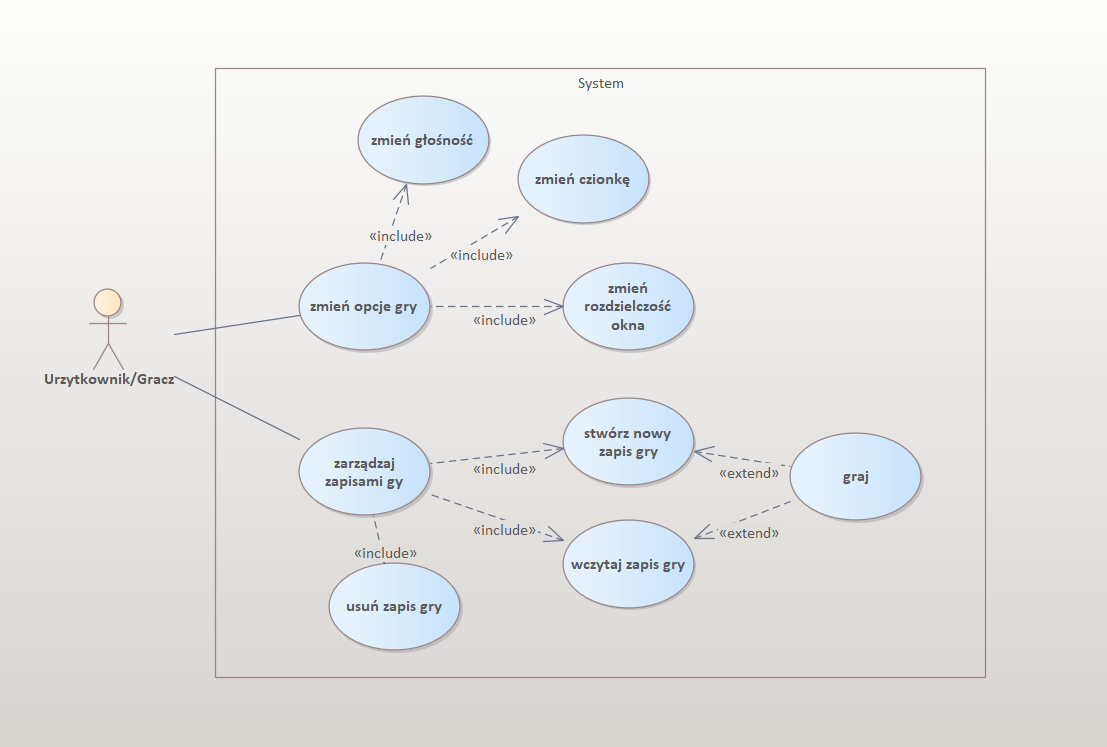
\includegraphics[width=\textwidth]{useCaseDiagram.png}
     \captionof{figure}{Diagram przypadków użycia}
\end{center}
\subsection{Wymagania funkcjonalne i niefunkcjonalne}
\subsubsection{Wymagania funkcjonalne}
Mapa:
\begin{itemize}
    \item proceduralna generacja mapy i obiektów oraz stworów znajdujące się na niej
    \item możliwość ustawienia wielkości generowanej mapy oraz ilości generowanych obiektów i stworów
    \item mapa podzielona na biomy\footnote{biom - obszar charakteryzujący się występowaniem predefiniowanych obiektów i stworów w ustalonych ilościach, np. biom "łąka"\space charakteryzuje się obfitym występowaniem wysokich traw i sporadycznym występowaniem drzew, a biom "las"\space zawiera w sobie wiele drzew i zwierząt takich jak jelenie i dziki.\cite{medium:biome}} różniące się ilością oraz rodzajem generowanych na nich obiektów i stworów
\end{itemize}
Stan gry:
\begin{itemize}
    \item możliwość zapisania stanu gry
    \item możliwość wczytania stanu gry z zapisu
    \item możliwość usunięcia zapisu stanu gry
\end{itemize}
Obiekty:
\begin{itemize}
    \item występowanie obiektów blokujących ruch postaci gracza i stworów
    \item występowanie obiektów świecących w nocy
    \item występowanie obiektów które są animowane
    \item zniszczone obiekty pozostawiają po sobie przedmioty
    \item obiekty mogą być niszczone wyłącznie przy pomocy odpowiedniego narzędzia
\end{itemize}
System dnia i nocy:
\begin{itemize}
    \item system pór dnia, kolejno: poranek, dzień, wieczór, noc
    \item system pór roku wpływających na długość poszczególnych pór dnia
\end{itemize}
Stwory:
\begin{itemize}
    \item stwory reagują na obecną porę dnia
    \item stwory mają odmienne wzorce zachowań, są: pasywne, neutralne lub agresywne
    \item występowanie stworów które są animowane
    \item występowanie stworów wydających dźwięki
\end{itemize}
Rozgrywka:
\begin{itemize}
    \item gracz jest w stanie poruszać postacią po mapie przy pomocy klawiatury lub myszy
    \item gracz jest w stanie wchodzić w interakcje z obiektami i stworami
    \item postać gracza może tracić i zyskiwać punkty życia i głodu
    \item postać gracza wraz z upływem czasu traci punkty głodu, a po całkowitej utracie punktów głodu zaczyna tracić punkty życia
    \item po utracie wszystkich punktów życia gracz przegrywa i nie może kontynuować gry na bieżącym zapisie gry
    \item postać gracza posiada ekwipunek, w którym może przechowywać przedmioty
    \item postać gracza może być wyposażona w narzędzie oraz zbroję
    \item możliwość ustawiania głośności gry
    \item głośność dźwięków zależy od odległości źródła dźwięku od gracza
    \item muzyka w grze zmienia się po przejściu z menu do gry
\end{itemize}
Interfejs:
\begin{itemize}
    \item występowanie zegara pokazującego obecny czas w grze, dzień i porę roku
    \item wizualne przedstawienie ilości punktów życia i głodu gracza
    \item animowane zmiany wartości punktów życia i głodu
    \item wizualne przedstawienie ekwipunku gracza
\end{itemize}

\subsubsection{Wymagania niefunkcjonalne}
\begin{itemize}
    \item gra działa w 40 FPS\footnote{FPS - (ang. frames per second) liczba klatek na sekundę, liczba oznaczająca ile razy na sekundę odświeża się ekran\cite{wiki:fps}} przy minimalnych wymaganiach sprzętowych\footnote{procesor: 2GHz lub więcej; pamięć: 2GB RAM; miejsce na dysku: 100MB} i domyślnych ustawieniach gry\footnote{domyślne ustawienia wybierane podczas tworzenia nowej gry}
    \item dwa rodzaje czcionek, jedna stylizowana i jedna ułatwiającą czytanie
    \item okno gry może przyjąć jeden z 2 ustalonych rozmiarów: HD\footnote{rozdzielczość 1280px×720px}, FULL HD\footnote{rozdzielczość 1920px×1080px} lub przejść w tryb pełnoekranowy
    \item pliki zapisu stanu gry są w formacie JSON
    \item pojedynczy plik zapisu stanu gry nie przekracza 1MB
    \item wszystkie teksty w grze są napisane w języku angielskim
\end{itemize}

\newpage
\subsection{Diagram klas}
Projekt składa się z ponad 90 klas, które można podzielić na 5 głównych grup ze względu na ich funkcjonalność. Poniższy diagram przedstawia przynależność poszczególnych klas do odpowiednich grup, które zostaną szczegółowo opisane w dalszej części pracy, oraz wszystkie powiązania między nimi. 

\begin{center}
     \includesvg[width=\textwidth]{ClassDiagram/ClassDiagram.svg}
     \captionof{figure}{Diagram przedstawiający przynależność klas do głównych kategorii oraz ich powiązania}
\end{center}

\subsubsection{Menu}
Menu gry oferuje 4 widoki, gdzie każdy z nich ma swoją odpowiadającą klasę. Wszystkie te klasy dziedziczą po wspólnym interfejsie "Menu", który przechowuje informacje o tle menu, tekstach i przyciskach, które mają być wyświetlane, a także udostępnia im między innymi funkcję "drawMenu", która wyrysowywuje menu na ekranie, oraz funkcję "reinitializeMenu", która ponownie inicjalizuje wszystkie elementy menu, co jest niezbędne podczas zmiany rozmiarów okna aplikacji.

Teksty i przyciski stanowiące część menu są osobnymi instancjami klas "Text"\space oraz "Button", gdzie obie klasy przechowują informacje o pozycji, tekście i czcionce, oraz zawierają funkcję "draw"\space umożliwiającą bezpośrednie wyświetlanie ich na ekranie.

Klasa "Button"\space dodatkowo zawiera informacje o akcji, która ma zostać wykonana po wciśnięciu oraz w odróżnieniu od klasy "Tekst"\space zmienia kolor czcionki, gdy użytkownik wskazuje na przycisk kursorem. Nadrzędnym elementem kontrolującym przechodzenie po poszczególnych widokach menu jest klasa "MenuController", to w niej znajduje się funkcja "menuLoop", która wykrywa akcje użytkownika takie jak ruch myszą lub wciśnięcie przycisku, oraz poprawnie na nie reaguje wyświetlając animacje oraz aktywując przyciski.

Gdy gracz nie podejmuje żadnych akcji w menu program na nie oczekuje nie obciążając procesora. Szczególnym widokiem menu jest widok tworzenia nowej gry reprezentowany przez klasę "CreateGame", która poza dziedziczeniem po klasie "Menu"\space dodatkowo korzysta z funkcji "generateMap", udostępnianej przez plik "GenerateMap", tworzącej zawartość nowego pliku zapisu gry.

\begin{center}
     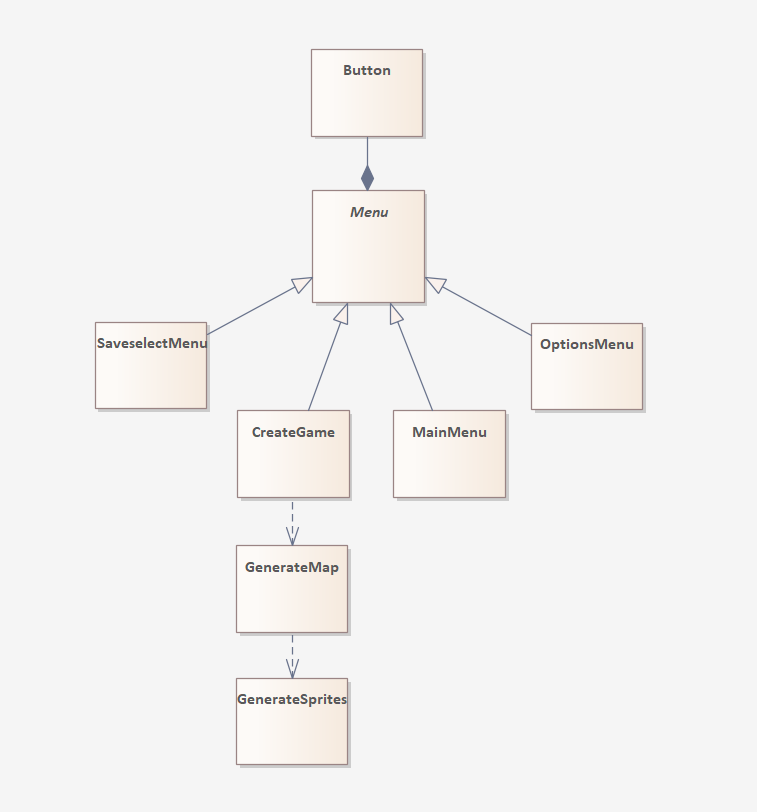
\includegraphics[width=\textwidth]{ClassDiagram/ClassDiagramMenu.png}
     \captionof{figure}{Fragment diagramu klas przedstawiający klasy powiązane z menu}
\end{center}

\subsubsection{Stwory}
Podstawową klasą zajmującą się zachowaniem stworów jest klasa "Entity". Przechowuje ona informacje o ich położeniu w świecie gry, wyglądzie, kierunku w którym są zwrócone oraz statystykach takich jak: prędkość poruszania się, liczba maksymalnych i obecnych punktów życia czy zasięg ataku stwora. Poza przechowywaniem informacji ta klasa zajmuje się również niezbędną logiką odpowiadającą za poruszanie się stwora, zmiany ilości punktów życia, zarządzanie stanem, wyświetlanie odpowiedniej grafiki oraz wywoływaniem nałożonych na niego efektów.

Postać gracza jest szczególnym przypadkiem stwora ponieważ w odróżnieniu od pozostałych stworów ta dziedziczy bezpośrednio po klasie "Entity". Reszta stworów dziedziczy po klasie "Mob", odpowiadającej za losowe poruszanie się stwora, który nie jest kontrolowany przez gracza.

Klasa "Mob"\space stanowi interfejs dla klas "AggressiveMob"\space oraz "PassiveMob", które rozszerzają wzorce zachowań stwora. Pierwsza z nich stanowi interfejs dla wszystkich mobów z natury agresywnych, czyli takich które atakują wszystkie pobliskie stwory nienależące do tej samej klasy. Poza logiką klasa ta przechowuje również informacje o sile oraz częstotliwości ataku stwora.

Z kolei klasa "PassiveMob"\space przechowuje logikę opisującą wzorce zachowań stworów pasywnych, czyli takich które nie walczą, a zamiast tego uciekają przed innymi stworami nienależącymi do tej samej klasy.

Poza tymi dwoma wzorcami zachowań jest jeszcze trzeci zdefiniowany w klasie "NeutralMob", który opisuje zachowanie stworów które są neutralne względem innych stworów tak długo jak nie zostaną zaatakowane, jeśli takowy stwór zostanie zaatakowany to zacznie się bronić atakując napastnika.

Ostatnim interfejsem związanym ze stworami jest klasa "AnimatedEntity", która dodaje logikę związaną z animacją poruszania się stwora.

\begin{center}
     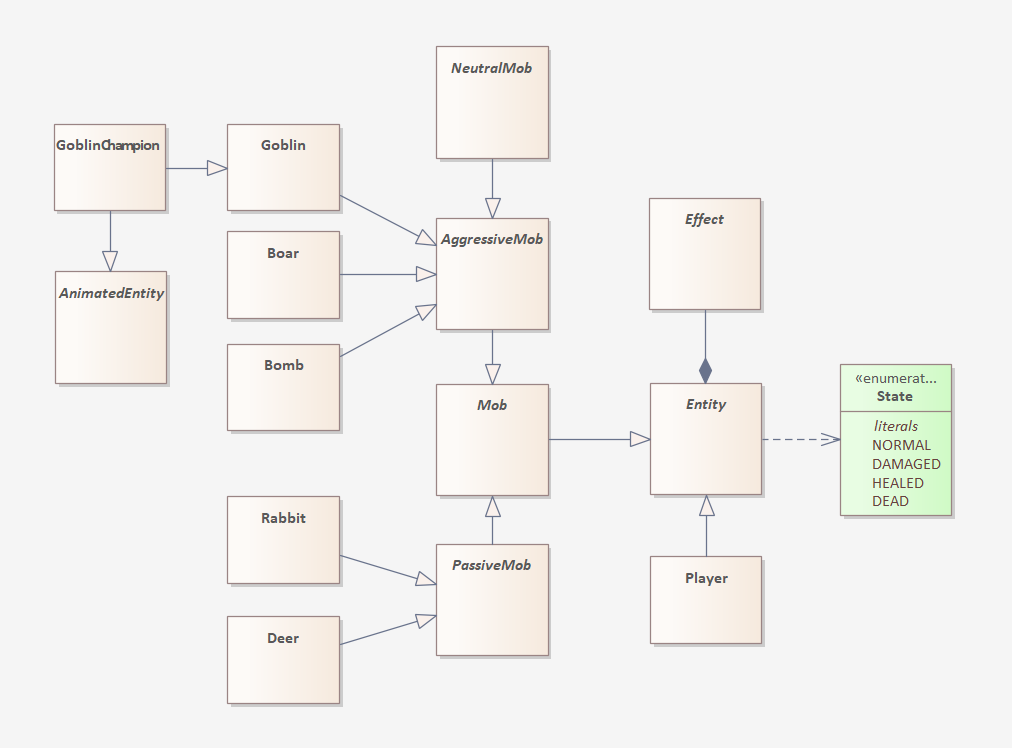
\includegraphics[width=\textwidth]{ClassDiagram/ClassDiagramEntity.png}
     \captionof{figure}{Fragment diagramu klas przedstawiający klasy powiązane ze stworami}
\end{center}

% \begin{center}
%      \includesvg[width=\textwidth]{ClassDiagram/ClassDiagramEntity.svg}
%      \captionof{figure}{Fragment diagramu klas przedstawiający klasy powiązane ze stworami}
% \end{center}

\subsubsection{Obiekty}
Obiekty są bytami znacznie prostszymi niż stwory, nie mogą się poruszać, ani nie mają złożonych wzorców zachowań. Głównym interfejsem po którym dziedziczą wszystkie obiekty jest klasa "Object". Przechowuje ona informacje o położeniu obiektu w świecie gry, jego wyglądzie, maksymalnej oraz obecnej ilości punktów wytrzymałości oraz typie narzędzia które jest potrzebne aby zniszczyć dany obiekt.

Po zniszczeniu obiekt może pozostawić po sobie przedmioty które następnie gracz może zebrać. Z niektórymi obiektami takimi jak wysoka trawa czyli instancjami klasy "Grass"\space gracz może wchodzić w interakcje bez potrzeby niszczenia ich. Wspomniana wysoka trawa może zostać przez gracza zebrana, przez co gracz otrzyma przedmiot, a trawa wejdzie w stan odrastania aby po ustalonym czasie wrócić do pierwotnej postaci.

Innym ciekawym obiektem jest królicza nora "RabbitHole", która przechowuje w sobie do trzech królików, które wracają do niej na wieczór i wychodzą z niej rano, a w przypadku śmierci któregoś z nich odradzają się po ustalonym czasie. Warto również wspomnieć o drzewach: "SmallTree", "MediumTree", "LargeTree"\space i "Snag", które z czasem zmieniają swoje stadium rozwoju dając wrażenie żywego ekosystemu.

Większość obiektów blokuje ruch stworów, są to obiekty dziedziczące po klasie "CollisionObject". Istnieją również obiekty które świecą w ciemności, te z kolei dziedziczą po klasie "Glowing". Niektóre obiekty są animowane i dziedziczą po klasie "AnimatedObject", która przechowuje w sobie wszystkie klatki animacji i zajmuje się poprawnym wyświetlaniem ich.

\begin{center}
     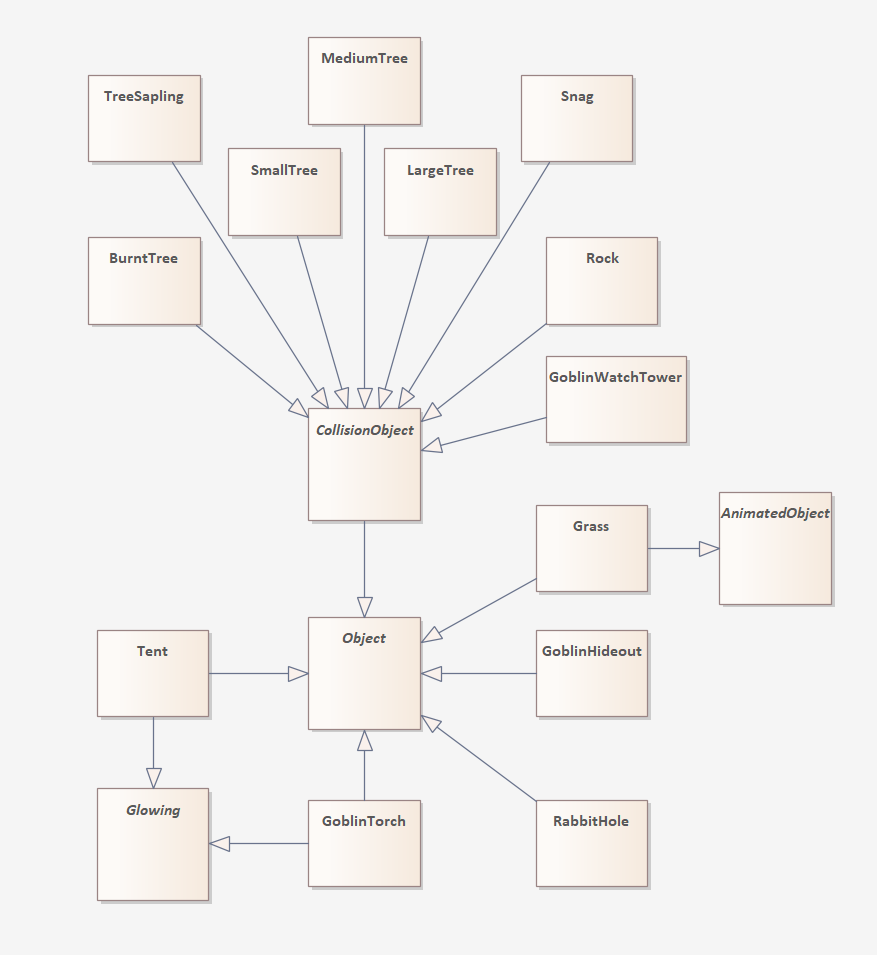
\includegraphics[width=\textwidth]{ClassDiagram/ClassDiagramObject.png}
     \captionof{figure}{Fragment diagramu klas przedstawiający klasy powiązane z obiektami}
\end{center}

\subsubsection{Przedmoty}
Wszystkie przedmioty dziedziczą po klasie "Item", która przechowuje informacje o ich wyglądzie, nazwie oraz pozycji w świecie gry. Przedmioty mogą również dziedziczyć po klasach "Tool"\space oraz "Armor", co sprawia że gracz może umieścić je w specjalnych miejscach w swoim ekwipunku i korzystać z ich umiejętności.

Przedmioty klasy "Tool"\space to narzędzia, które dodatkowo przechowują informacje o swojej sile ataku, wydajności oraz maksymalnej i obecnej wytrzymałości. Gracz w danej chwili może korzystać wyłącznie z jednego narzędzia, które daje mu możliwość niszczenia odpowiadających obiektów, lub zadaje zwiększone obrażenia.

Przedmioty klasy "Armor"\space stanowią zbroje i dodatkowo przechowują informacje o ustalonej ilości obrażeń które zbroja blokuje oraz o procencie obrażeń które zbroja blokuje. Podobnie jak w przypadku narzędzi gracz w danej chwili może korzystać wyłącznie z jednej zbroi. Poza możliwością użytkowania niektórych przedmiotów występują również przedmioty jednorazowe takie jak jedzenie "SmallMeat"\space i "LargeMeat", które gracz może wykożystać aby się nasycić i uleczyć część utraconych punktów życia.

\begin{center}
     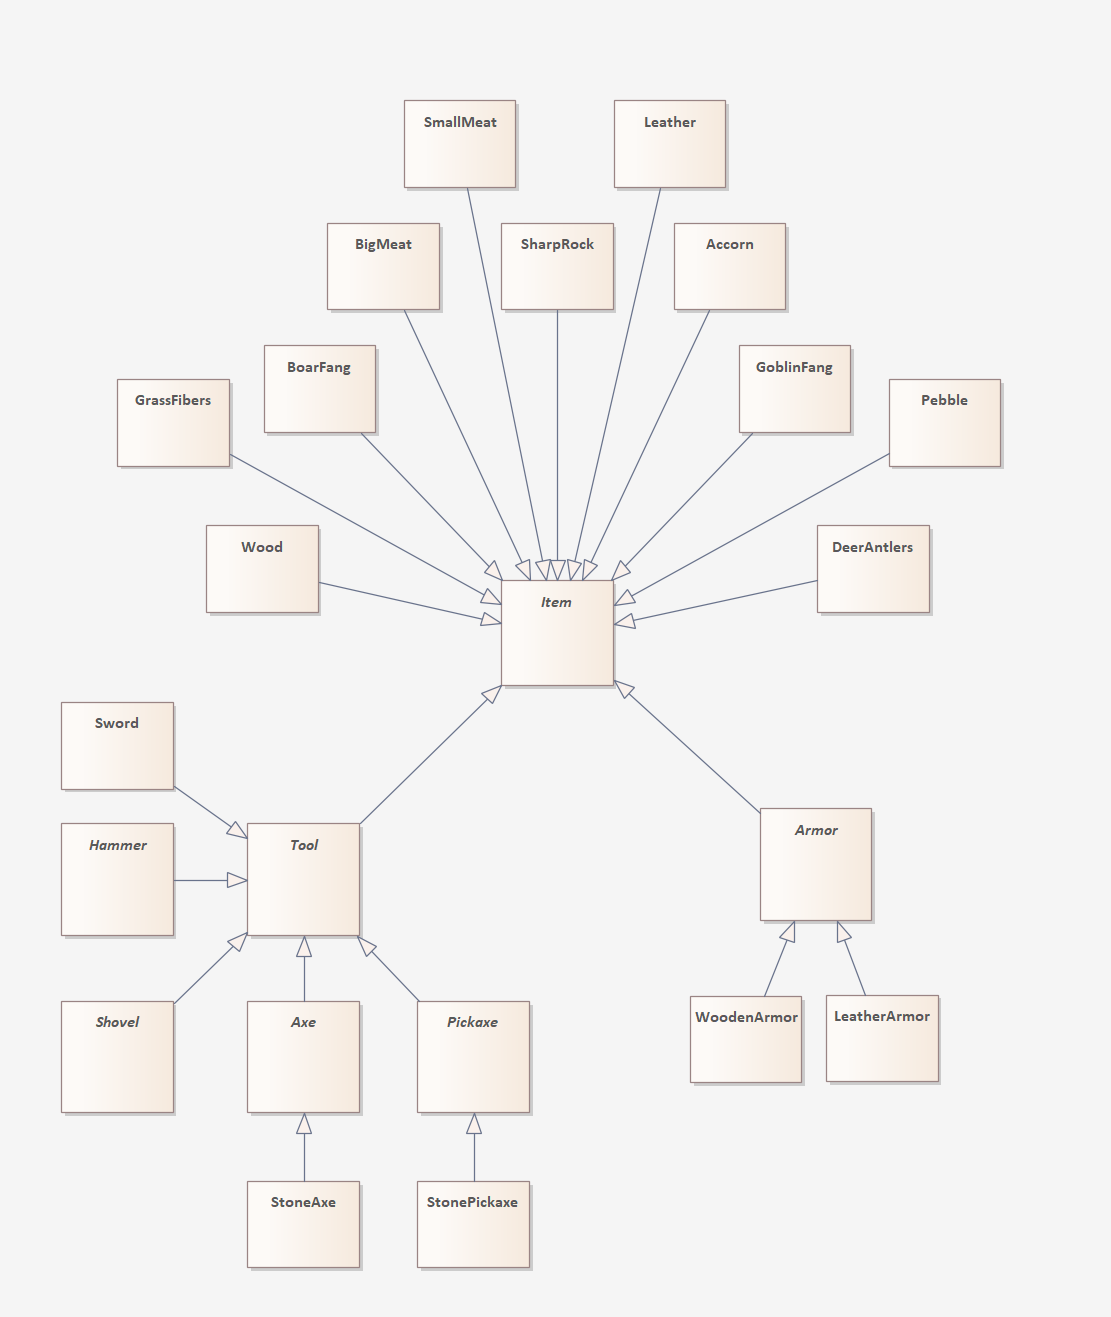
\includegraphics[width=\textwidth]{ClassDiagram/ClassDiagramItem.png}
     \captionof{figure}{Fragment diagramu klas przedstawiający klasy powiązane z przedmiotami}
\end{center}

\subsubsection{Gra}
Klasa "Game"\space jest najważniejszą ze wszystkich klas. Jest łącznikiem pomiędzy pozostałymi klasami i zawiera w sobie główną pętlę gry. Poza tym zajmuje się inicjalizacją gry, poprzez tworzenie instancji odpowiednich klas korzystając z danych z pliku zapisu, a także za zapisywanie bieżącego stanu gry.

Podczas tworzenia nowych instancji klas korzystających z obrazów i dźwięków, które trzeba załadować z pamięci komputera, w celu uniknięcia konieczności wielokrotnego wczytywania ich stworzyliśmy klasy "LoadedImages"\space i "LoadedSounds", które przechowują w sobie wszystkie grafiki i dźwięki, z których inne klasy mogą korzystać, co sprawia że gra wczytuje się szybciej, a rozgrywka jest płynniejsza.

Kolejną klasą będącą częścią gry jest "CameraSpriteGroup", która odpowiedzialna jest za rysowanie sprite'ów\footnote{sprite - dwuwymiarowy obrazek rastrowy używany w systemach grafiki dwuwymiarowej i 2,5-wymiarowej, który po przesunięciu i ewentualnym przeskalowaniu jest przenoszony na ekran wyświetlacza.\cite{wiki:sprite}} na ekranie tak aby w centrum okna aplikacji zawsze była postać gracza. Odpowiada ona także za wyrysowywanie na ekranie efektów pogodowych oraz efektu ciemności, z uwzględnieniem źródeł światła. Dodatkowo jak w wielu innych grach\footnote{np. Minecraft, Counter-Strike, Roblox} istnieje możliwość wizualizacji hitbox'ów\footnote{domyślnie niewidzialny obszar wyznaczony w ramach sprite'a używany do detekcji kolizji w czasie rzeczywistym\cite{wiki:hitbox}} po wciśnięciu odpowiedniego przycisku. Korzystając z faktu że wszystkie sprite'y, a co za tym idzie wszystkie obiekty, stwory oraz przedmioty są powiązane z klasą "CameraSpriteGroup", owa klasa przy pomocy klasy "SavefileGroups"\space umożliwia zgromadzenie danych do pliku zapisu gry ze wszystkich sprite'ów.

Inną klasą przechowującą informacje o sprite'ach jest "ObstacleSprites". W odróżnieniu od "CameraSpriteGroup"\space ta klasa zawiera informacje wyłącznie o sprite'ach które blokują poruszanie się stworów, co umożliwia sprawne wykrywanie kolizji. Szczególnie ciekawą funkcją w tej klasie jest "getNearbyTiles", która dostaje w parametrze pozycję w świecie gry i zwraca listę najbliższych fragmentów mapy świata, które blokują ruch, dzięki czemu wykrywanie kolizji jest znacznie usprawnione.

Kolejną klasą powiązaną z "Game"\space jest "UiSpriteGroup", która zajmuje się wyświetlaniem elementów interfejsu gry, takich jak zegar, ekwipunek oraz statystki gracza. Statystyki gracza są wyświetlane wykorzystując klasę "Bar", która wizualizuje je w postaci animowanego paska, a ekwipunkiem gracza zarządza klasa "Inventory". Dodatkowo inwentarz jest podzielony na mniejsze fragmenty, klasa "Slot", które mogą przechowywać dowolny przedmiot lub przedmiot wyłącznie określonej klasy.

Klasa "Game"\space zawiera w sobie dodatkowo klasę "DayCycle", zarządzającą obecnym czasem i dniem w świecie gry, kontrolując fazy dnia oraz pory roku. Dodatkowo przekazuje informacje o zmianie fazy dnia wszystkim klasą dziedziczącym po "DayPhaseListener".

Ostatnią klasą będącą częścią klasy "Game"\space jest "WeatherController", która zarządza pogodą w świecie gry.

\begin{center}
     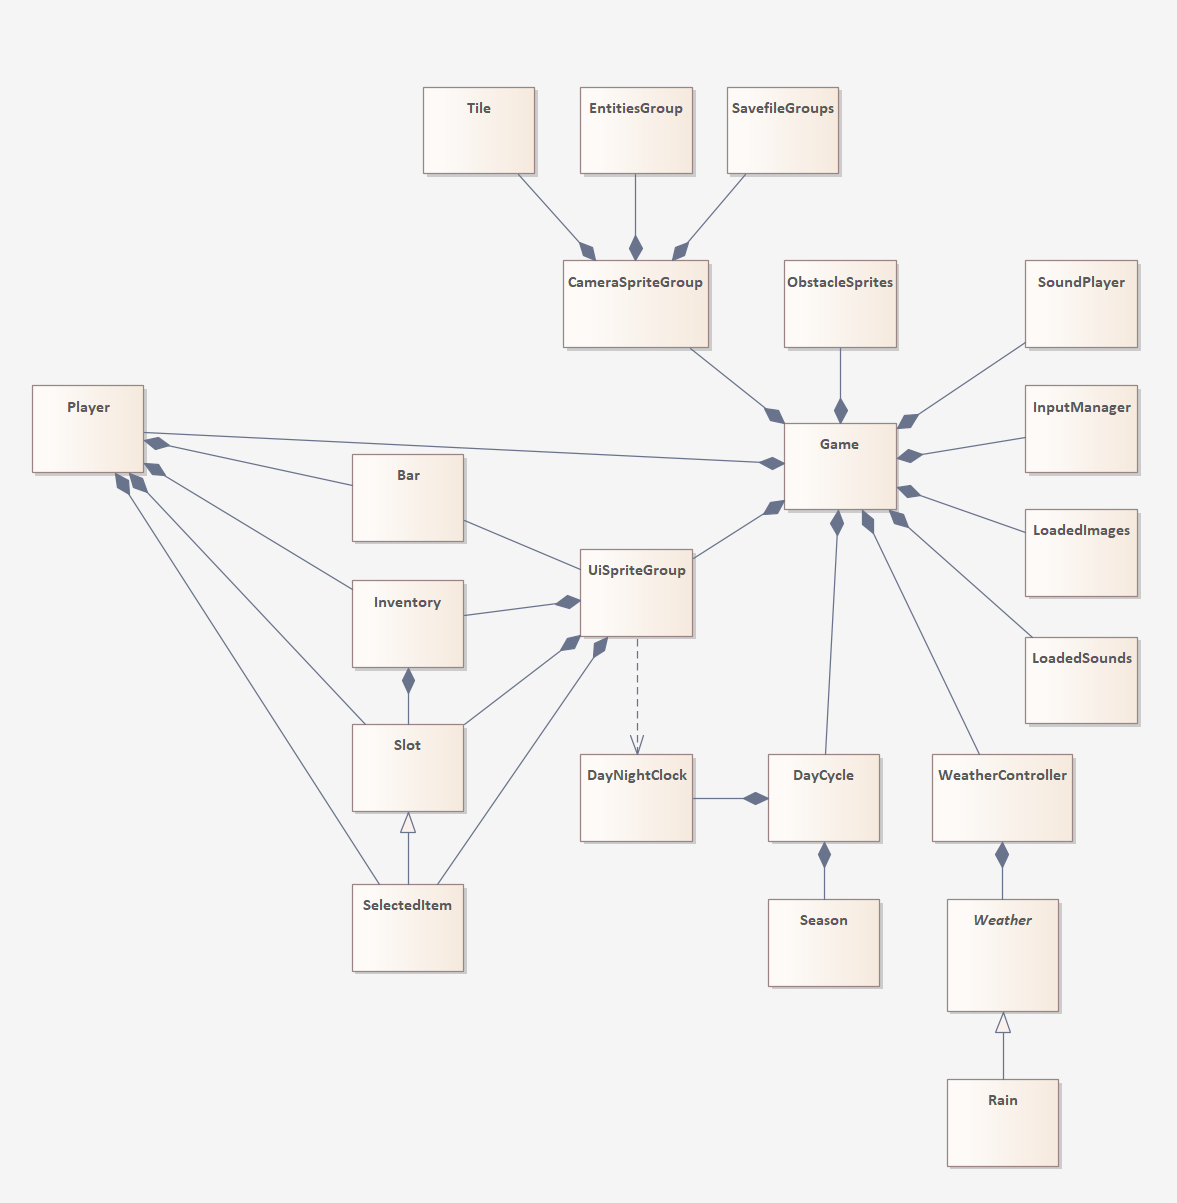
\includegraphics[width=\textwidth]{ClassDiagram/ClassDiagramGame.png}
     \captionof{figure}{Fragment diagramu klas przedstawiający klasy powiązane z główną klasą gry}
\end{center}

\newpage
\subsection{Schemat pliku zapisu}
Plik zapisu stanu gry jest w formacie JSON. Przechowuje informacje o nazwie zapisu gry, obecnym dniu oraz czasie w świecie gry, mapie świata gry w postaci listy list numerów id odpowiadających poszczególnym biomom oraz informacje o wszystkich obiektach, stworach, przedmiotach i ekwipunku gracza.\\
\begin{center}
    \begin{lstlisting}[language=jsonSchema]
{
    "savefileName": str
    "currentDay": int
    "currentTimeMs": int
    "map": [[int]]
    "sprites": [dict]
    {
        "Player": [dict]
        {
            "midbottom": [int, int]
            "currHealth": int
            "currHunger": float
            "inventoryData": dict
            {
                "inventory": dict
                {
                    "slotsItemData": [str | None]
                }
                "handSlot": str
                "bodySlot": str
            }
        }
        "*entityName": [dict]
        {
            "midbottom": [int, int]
            "currHealth": int
            "home": None (opcjonalnie)
            "isHomeless": bool (opcjonalnie)
        }
        "*objectName": [dict]
        {
            "midbottom": [int, int]
            "currentDurability": int
            "entitesDataList": [dict] (opcjonalnie)
            "daysFromEntitiesChange": int (opcjonalnie)
        }
        "*itemName": [dict]
        {
            "center": [int, int]
            "id": str
            "currDurability": int (opcjonalnie)
        }
    }
}
    \end{lstlisting}
    \captionof{figure}{Schemat zapisu pliku}
\end{center}
\subsection{Projekt interfejsu użytkownika}
\subsubsection{Menu}
Menu składa się z czterech widoków pełniących odmienne funkcje: menu główne, menu opcji, menu wyboru zapisu gry oraz menu tworzenia gry. Menu główne jest pierwszym widokiem który widzi użytkownik po uruchomieniu aplikacji. Z jego poziomu można przejść do menu wyboru zapisu gry, menu opcji lub zamknąć aplikację.
\begin{center}
     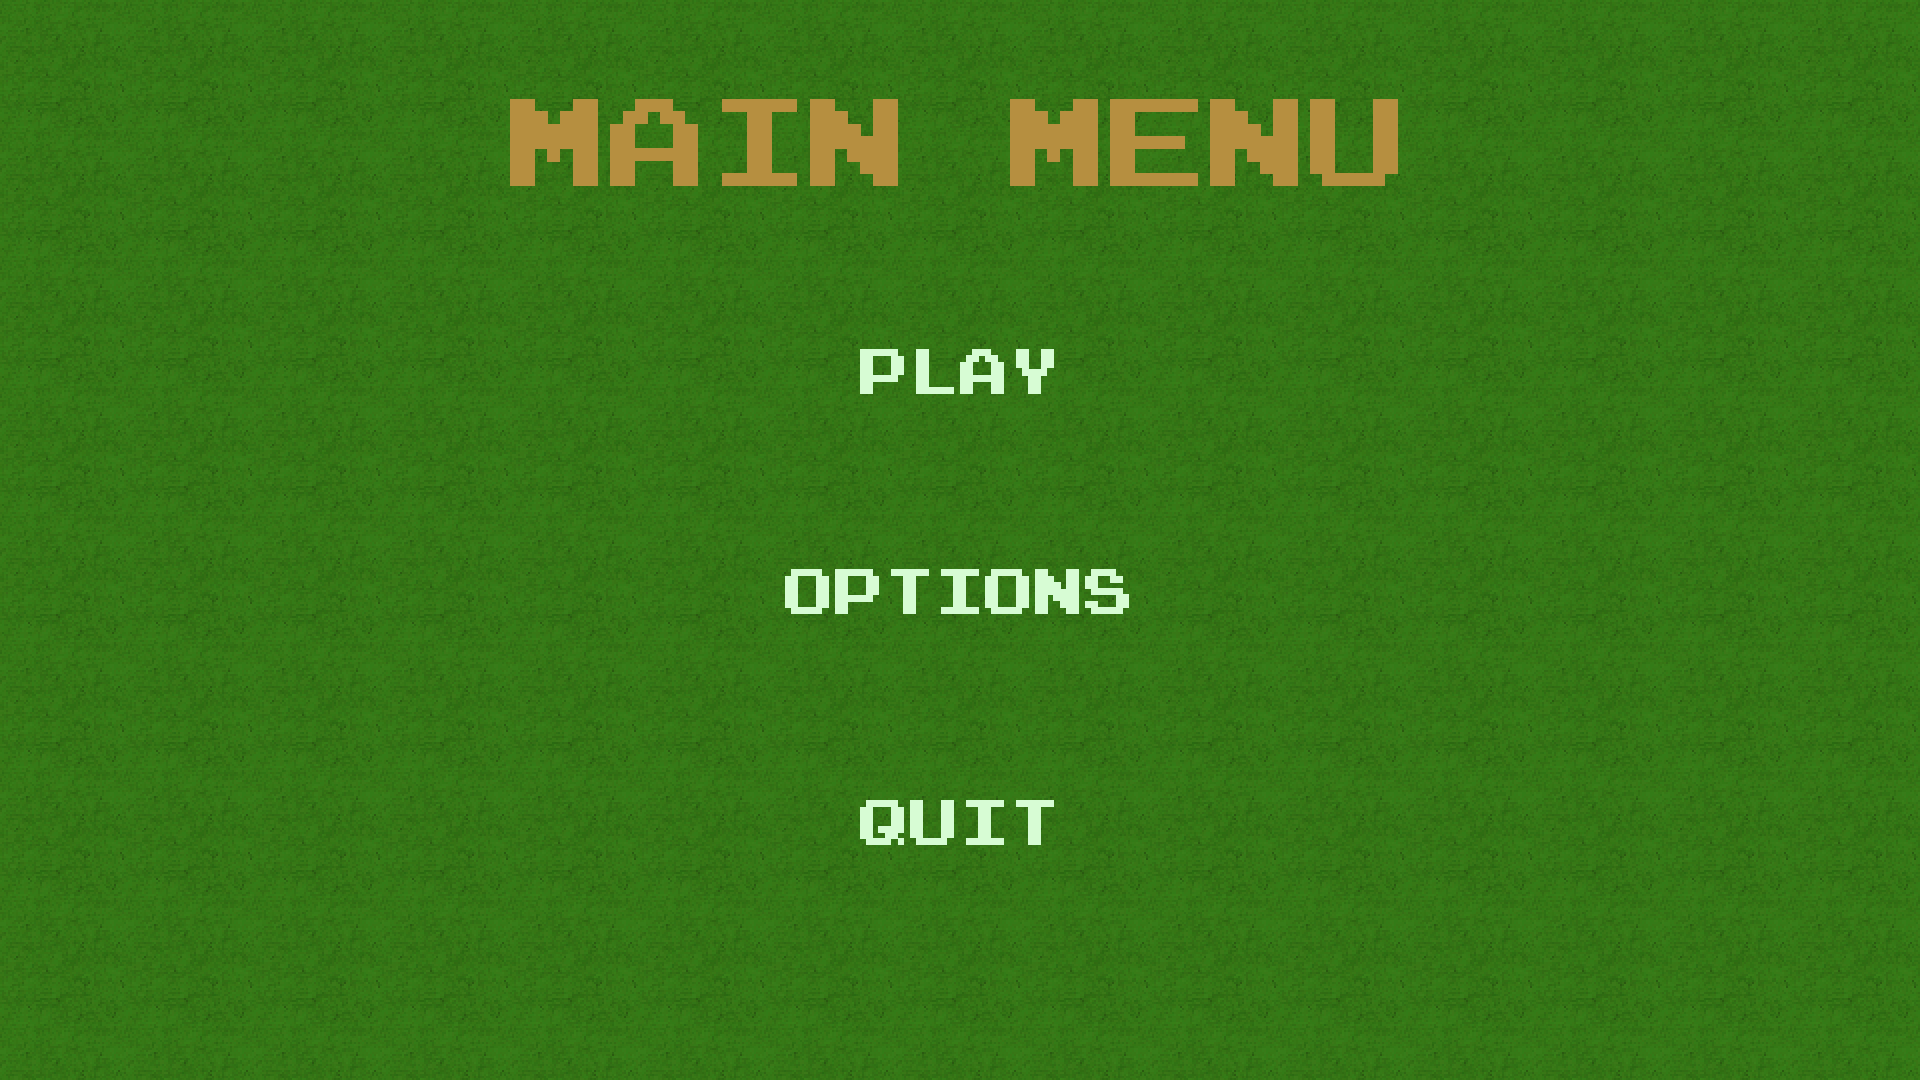
\includegraphics[width=\textwidth]{mainMenu.png}
     \captionof{figure}{Zrzut ekranu przedstawiający menu główne}
\end{center}
Menu opcji umożliwia dostosowanie parametrów gry według preferencji użytkownika. Będąc w tym menu można zmienić rodzaj czcionki ze stylizowanej na ułatwiającą czytanie, dostosować głośność muzyki oraz zmienić rozdzielczość okna gry.
\begin{center}
     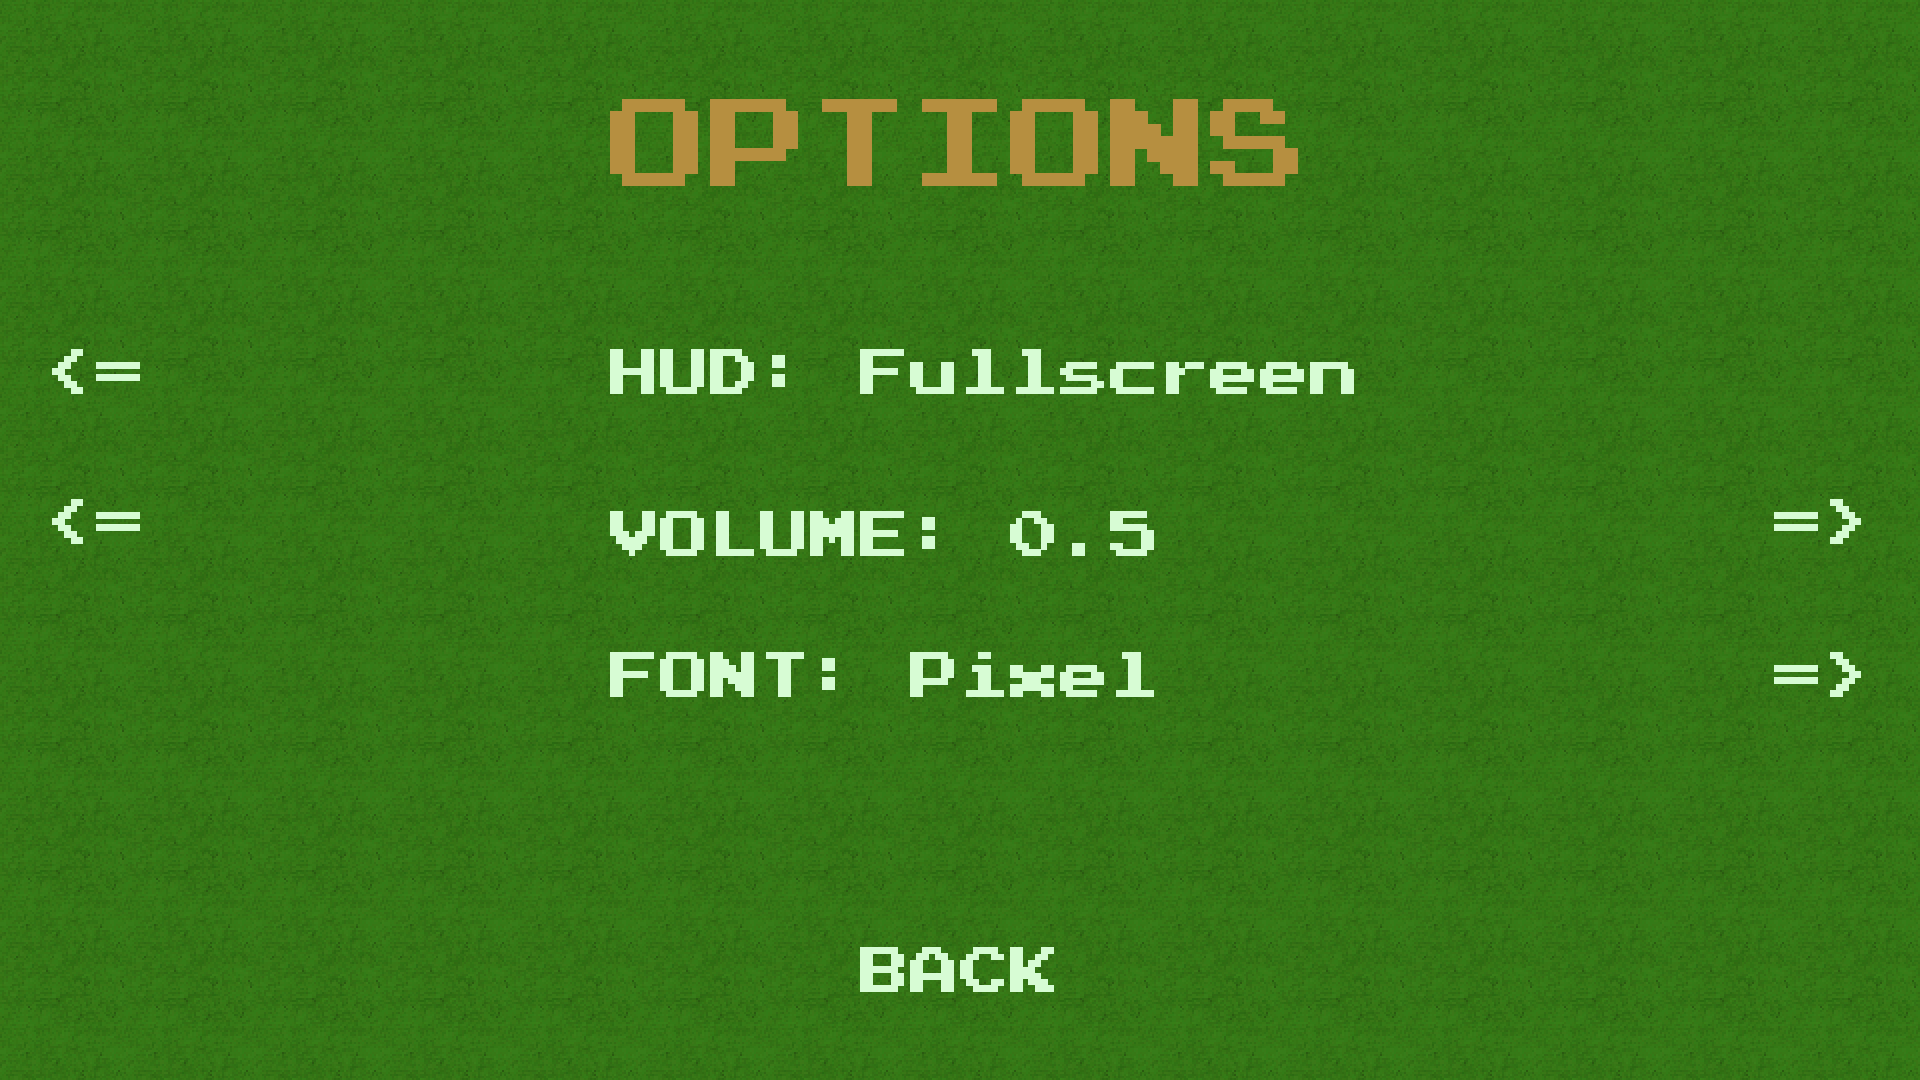
\includegraphics[width=\textwidth]{optionsMenu.png}
     \captionof{figure}{Zrzut ekranu przedstawiający menu opcji}
\end{center}
\begin{center}
     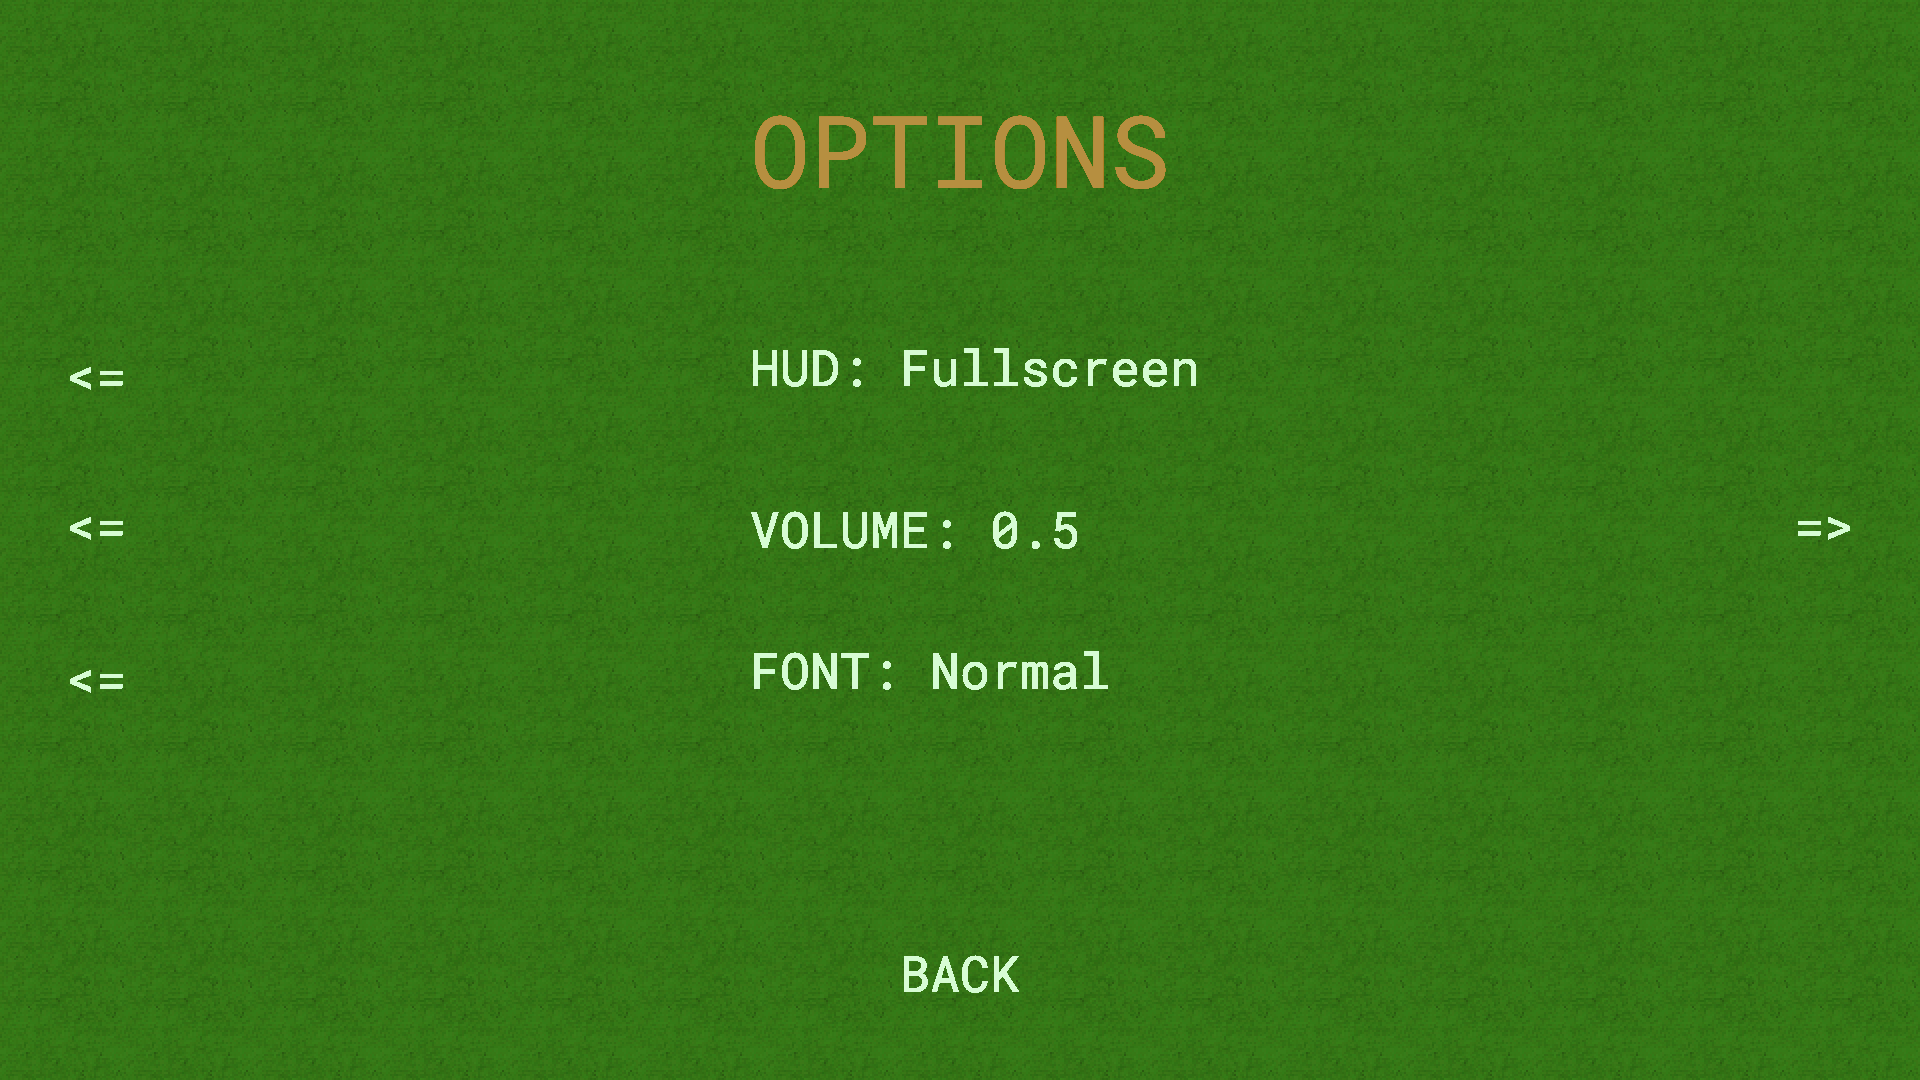
\includegraphics[width=\textwidth]{optionsMenuSecondFont.png}
     \captionof{figure}{Zrzut ekranu przedstawiający menu opcji po wyborze czcionki ułatwiającej czytanie}
\end{center}
Menu wyboru zapisu gry oferuje graczowi 3 miejsca na potencjalne zapisy gry. Z poziomu tego widoku można usunąć niechciane zapisy gry poprzez kliknięcie przycisku "X", który po wskazaniu na niego kursorem zmieni kolor na czerwony, znajdującego się po lewej stronie wybranego zapisu. Przycisk "X"\space wyświetla się wyłącznie przy miejscach na zapis gry które są obecnie zajęte. Z poziomu tego menu można również wczytać wybrany zapis gry poprzez kliknięcie na jego nazwę, co spowoduje uruchomienie gry. W przypadku gdy użytkownik kliknie na nazwę zapisu gry który nie jest obecnie zajęty zostanie on przekierowany do menu tworzenia gry.
\begin{center}
     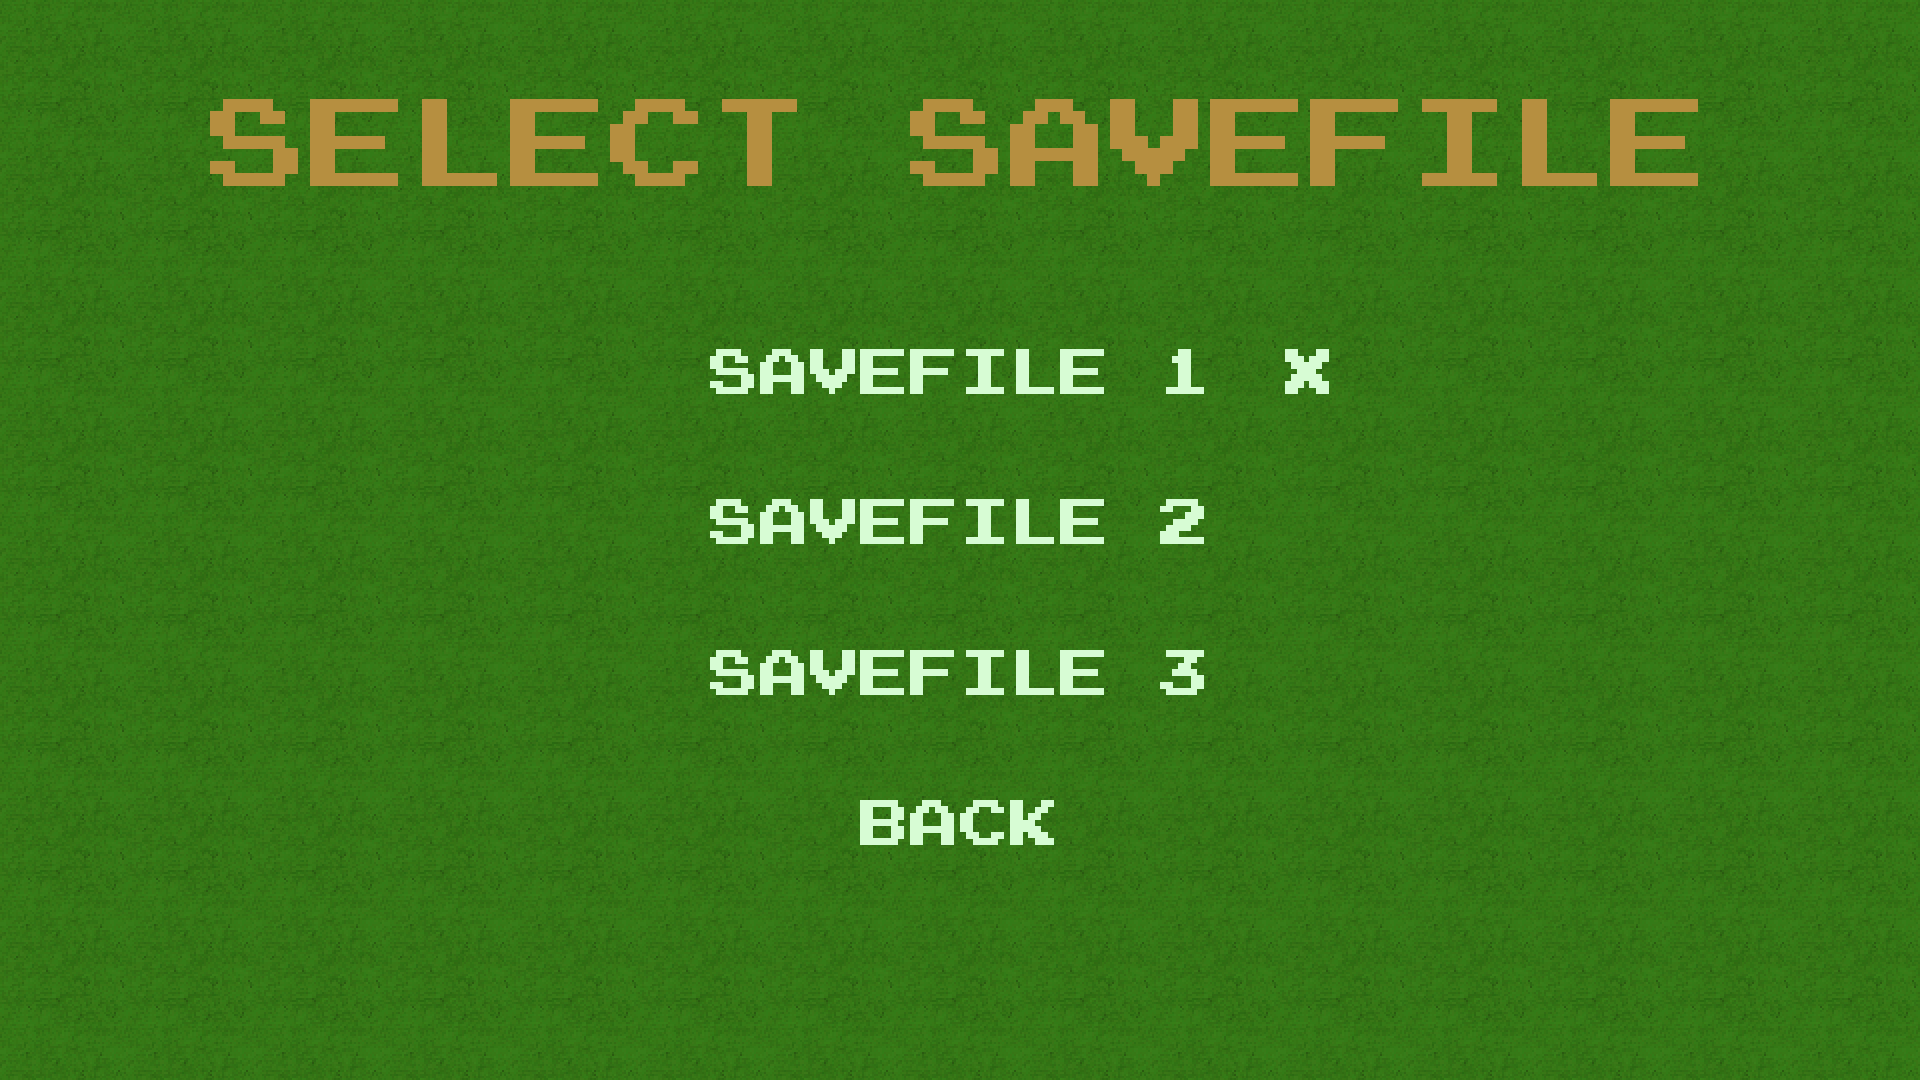
\includegraphics[width=\textwidth]{saveSelectMenu.png}
     \captionof{figure}{Zrzut ekranu przedstawiający menu wyboru zapisu gry}
\end{center}
Menu tworzenia gry pozwala użytkownikowi dostosować parametry swojego nowo generowanego świata według swojej wizji. Ten widok pozwala na zmianę wielkości mapy poprzez wybranie jednego z pięciu rozmiarów oraz zmianę ilości generowanych na niej obiektów i stworów, co bezpośrednio wpływa na poziom trudności rozgrywki. Po zakończeniu zmieniania ustawień użytkownik może kliknąć przycisk "CREATE GAME"\space który rozpocznie sekwencję generowania świata gry, a użytkownik zostanie przeniesiony do widoku ładowania.
\begin{center}
     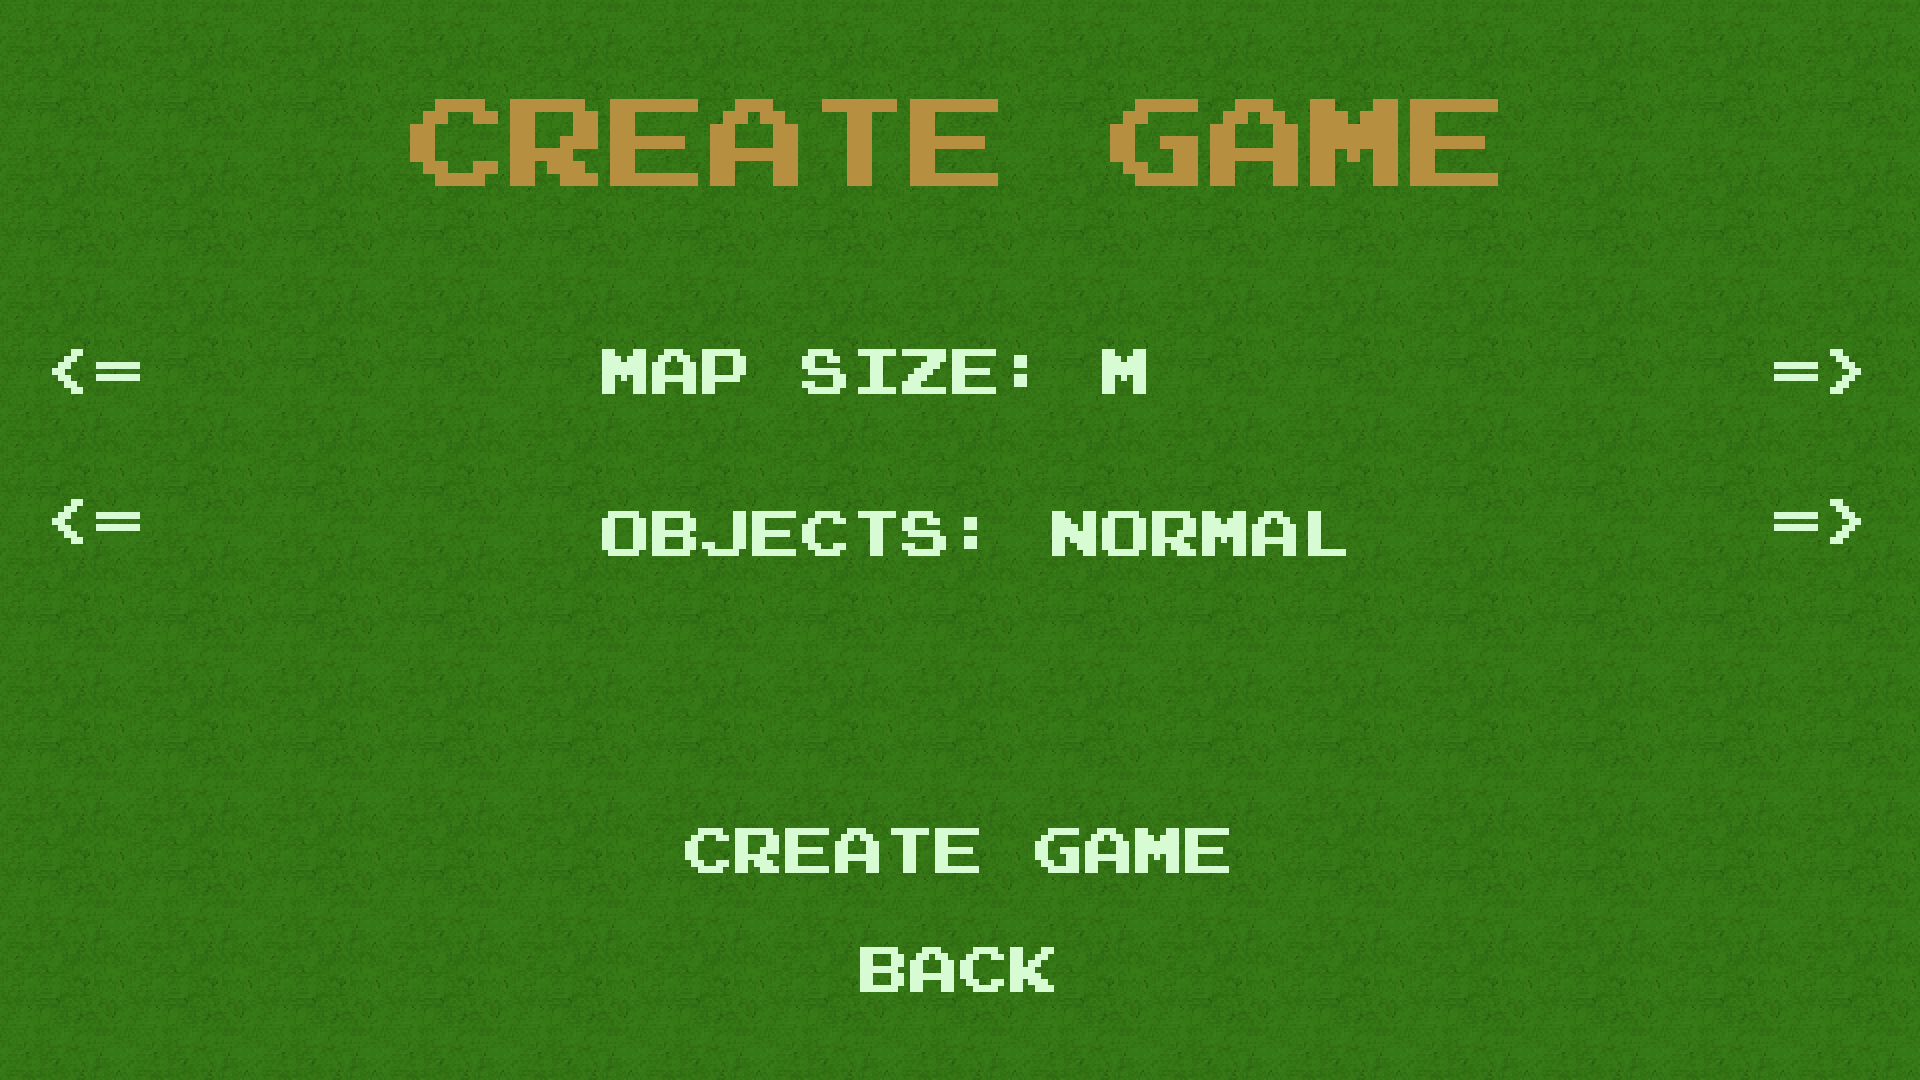
\includegraphics[width=\textwidth]{createGameMenu.png}
     \captionof{figure}{Zrzut ekranu przedstawiający menu tworzenia nowej gry}
\end{center}
W trakcie oczekiwania na stworzenie świata gry poprzez jego wygenerowanie lub załadowanie z zapisu gracz jest w stanie śledzić bieżący etap wczytywania gry za pomocą komunikatów wyświetlających się na ekranie.
\begin{center}
     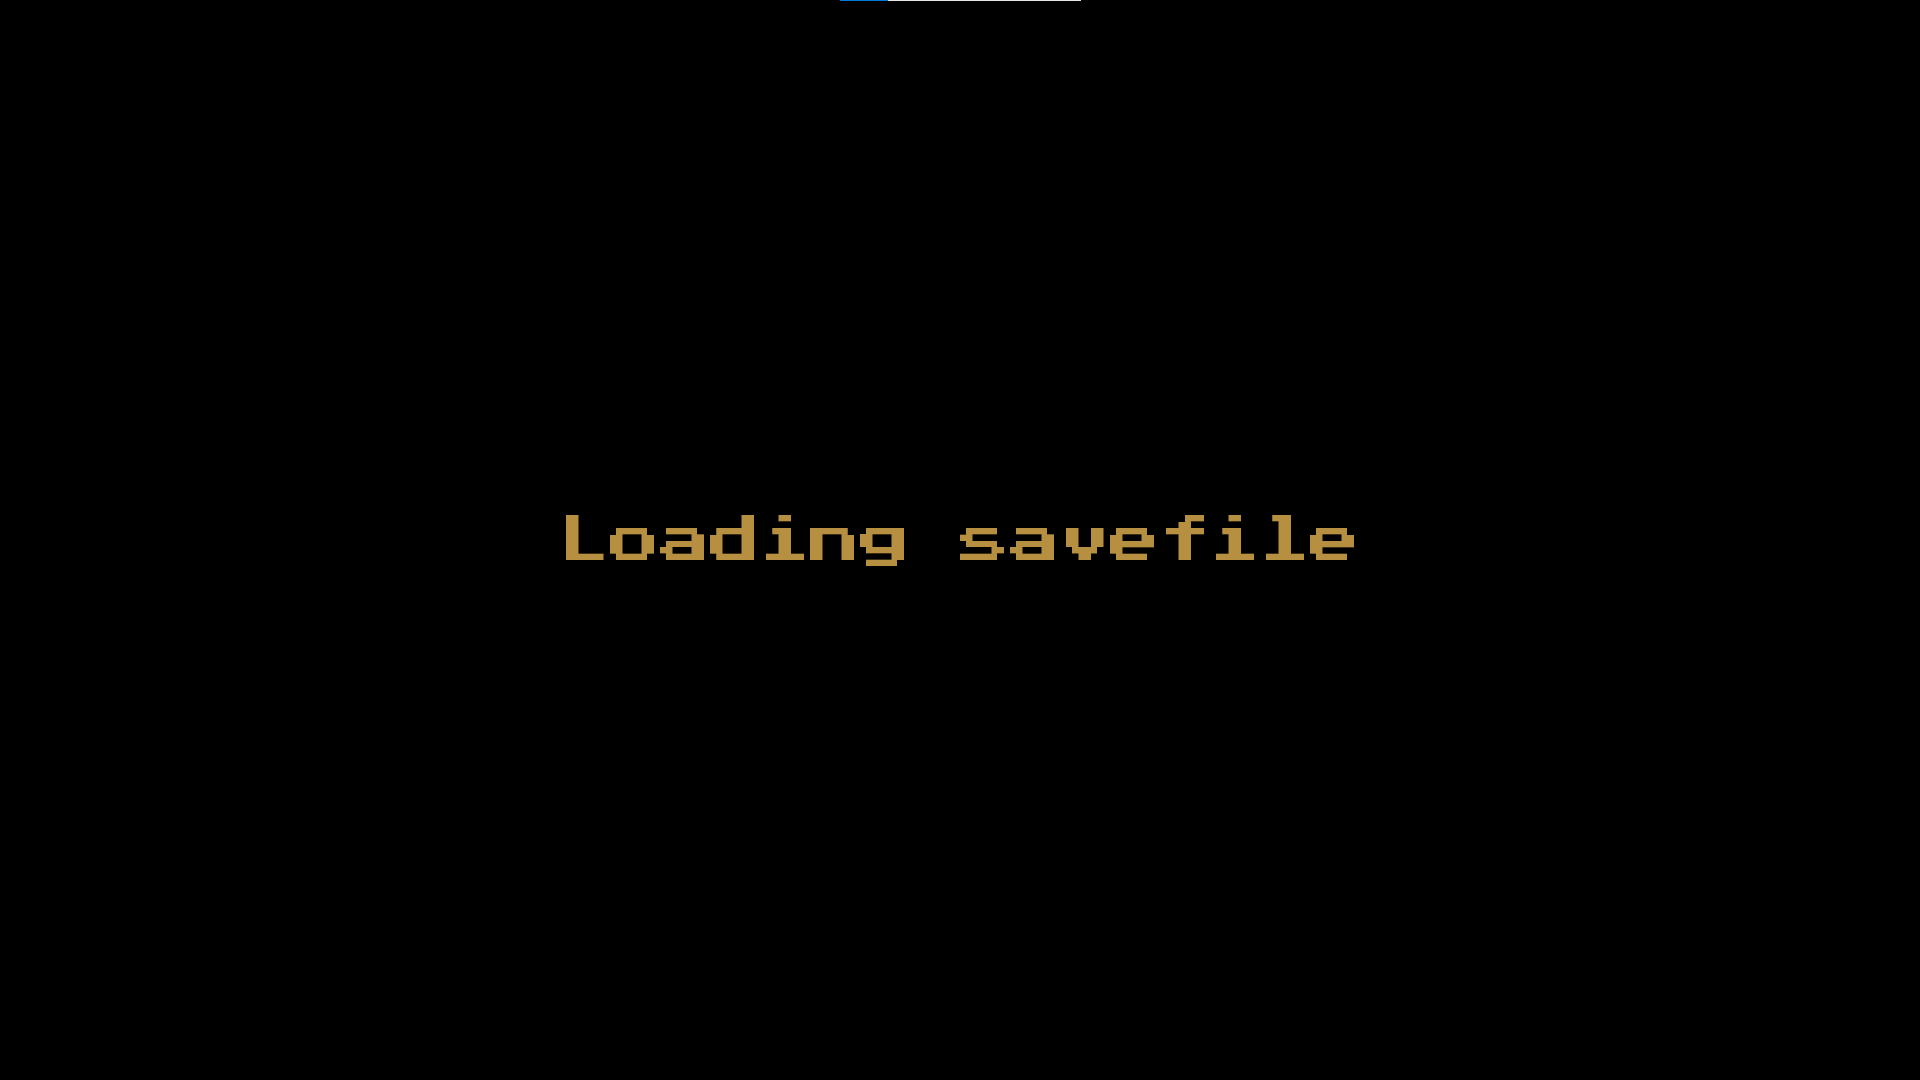
\includegraphics[width=\textwidth]{loadingView.png}
     \captionof{figure}{Zrzut ekranu przedstawiający menu ładowania gry}
\end{center}
\newpage
\subsubsection{Gra}
Interfejs użytkownika w grze składa się z trzech głównych elementów: zegara, ekwipunku i statystyk.  Czcionka użyta w grze odpowiada tej wybranej w menu opcji.

\begin{center}
     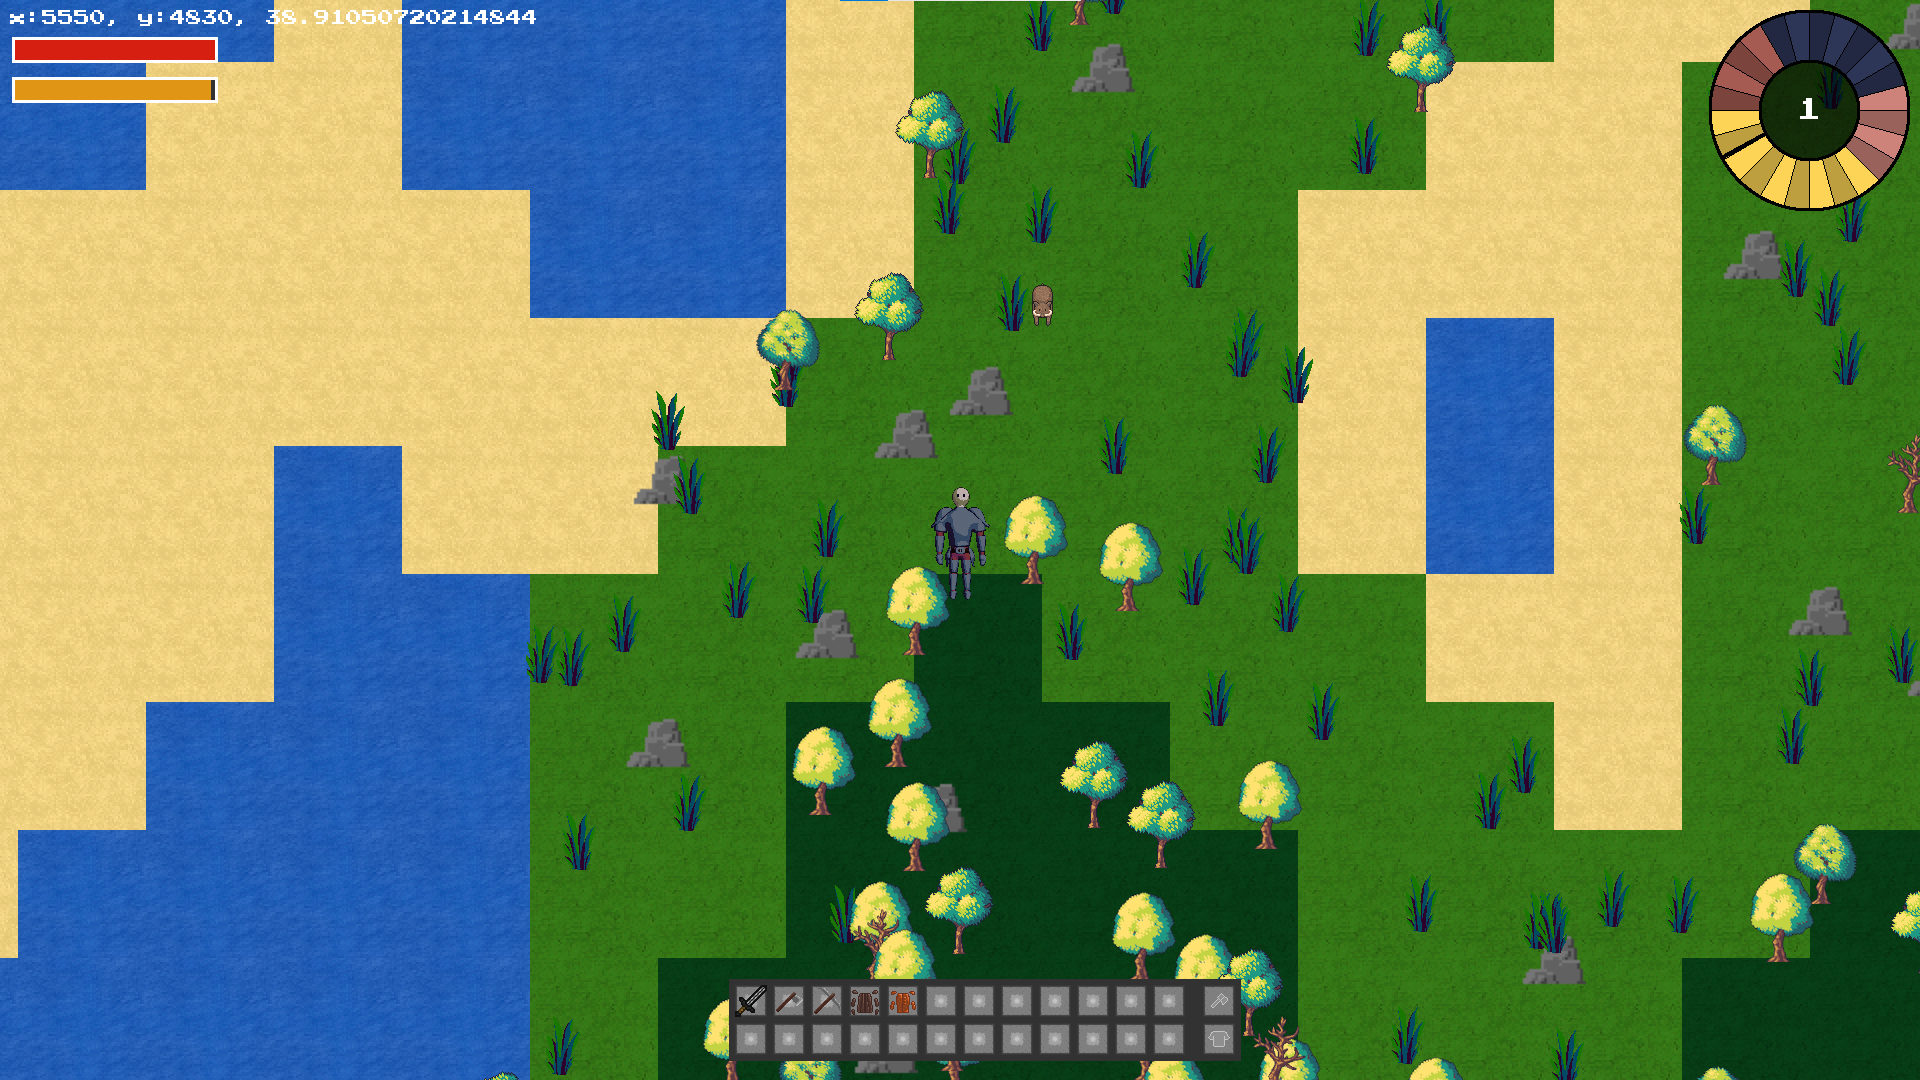
\includegraphics[width=\textwidth]{gra.png}
     \captionof{figure}{Zrzut ekranu przedstawiający grę}
\end{center}

Zegar znajduje się w górnym prawym rogu ekranu i jest podzielony na dwie części, półprzezroczysty środek, w którym wyświetla się numer dnia, oraz zewnętrzny pierścień, z którego można odczytać obecną godzinę i porę roku w świecie gry. Zewnętrzny pierścień podzielony jest na 24 segmenty symbolizujące godziny oraz wskazówkę. Dodatkowo każdy z segmentów ma przypisany jeden z czterech kolorów, które zmieniają się w zależności od obecnej pory roku, po których można rozpoznać jaką fazę dnia reprezentują.

\begin{center}
     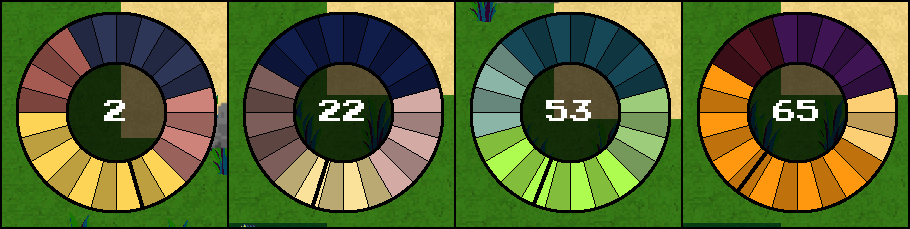
\includegraphics[width=\textwidth]{zegary.png}
     \captionof{figure}{Fragment ekranu przedstawiające zegar we wszystkich porach roku, kolejno od lewej: jesień, zima, lato, wiosna.}
\end{center}

\newpage

Ekwipunek gracza znajduje się w dolnej części ekranu i również jest podzielony na dwie główne części, gdzie pierwsza od lewej to plecak gracza, wyświetla on przedmioty które gracz posiada i może wykorzystać, a druga część to przedmioty z których postać gracza korzysta w obecnej chwili. W danym momencie gracz może wyposażyć swoją postać w wyłącznie jedno narzędzie oraz jedną ubranie.

\begin{center}
     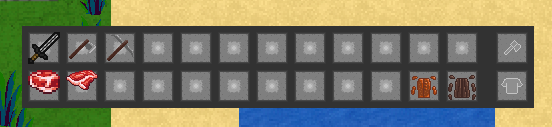
\includegraphics[width=\textwidth]{ekwipunek.png}
     \captionof{figure}{Fragment ekranu przedstawiający ekwipunek}
\end{center}

Statystyki wyświetlają się w górnym lewym rogu ekranu i składają się z animowanego paska życia i paska nasycenia, dokładnej pozycji postaci gracza w świecie gry oraz bieżącej ilości FPS\cite{wiki:fps}.

\begin{center}
     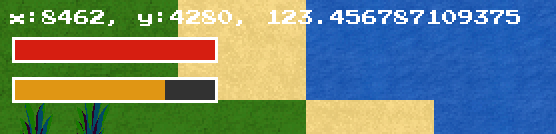
\includegraphics[width=\textwidth]{statystyki.png}
     \captionof{figure}{Fragment ekranu przedstawiający statystyki}
\end{center}
\begin{center}
     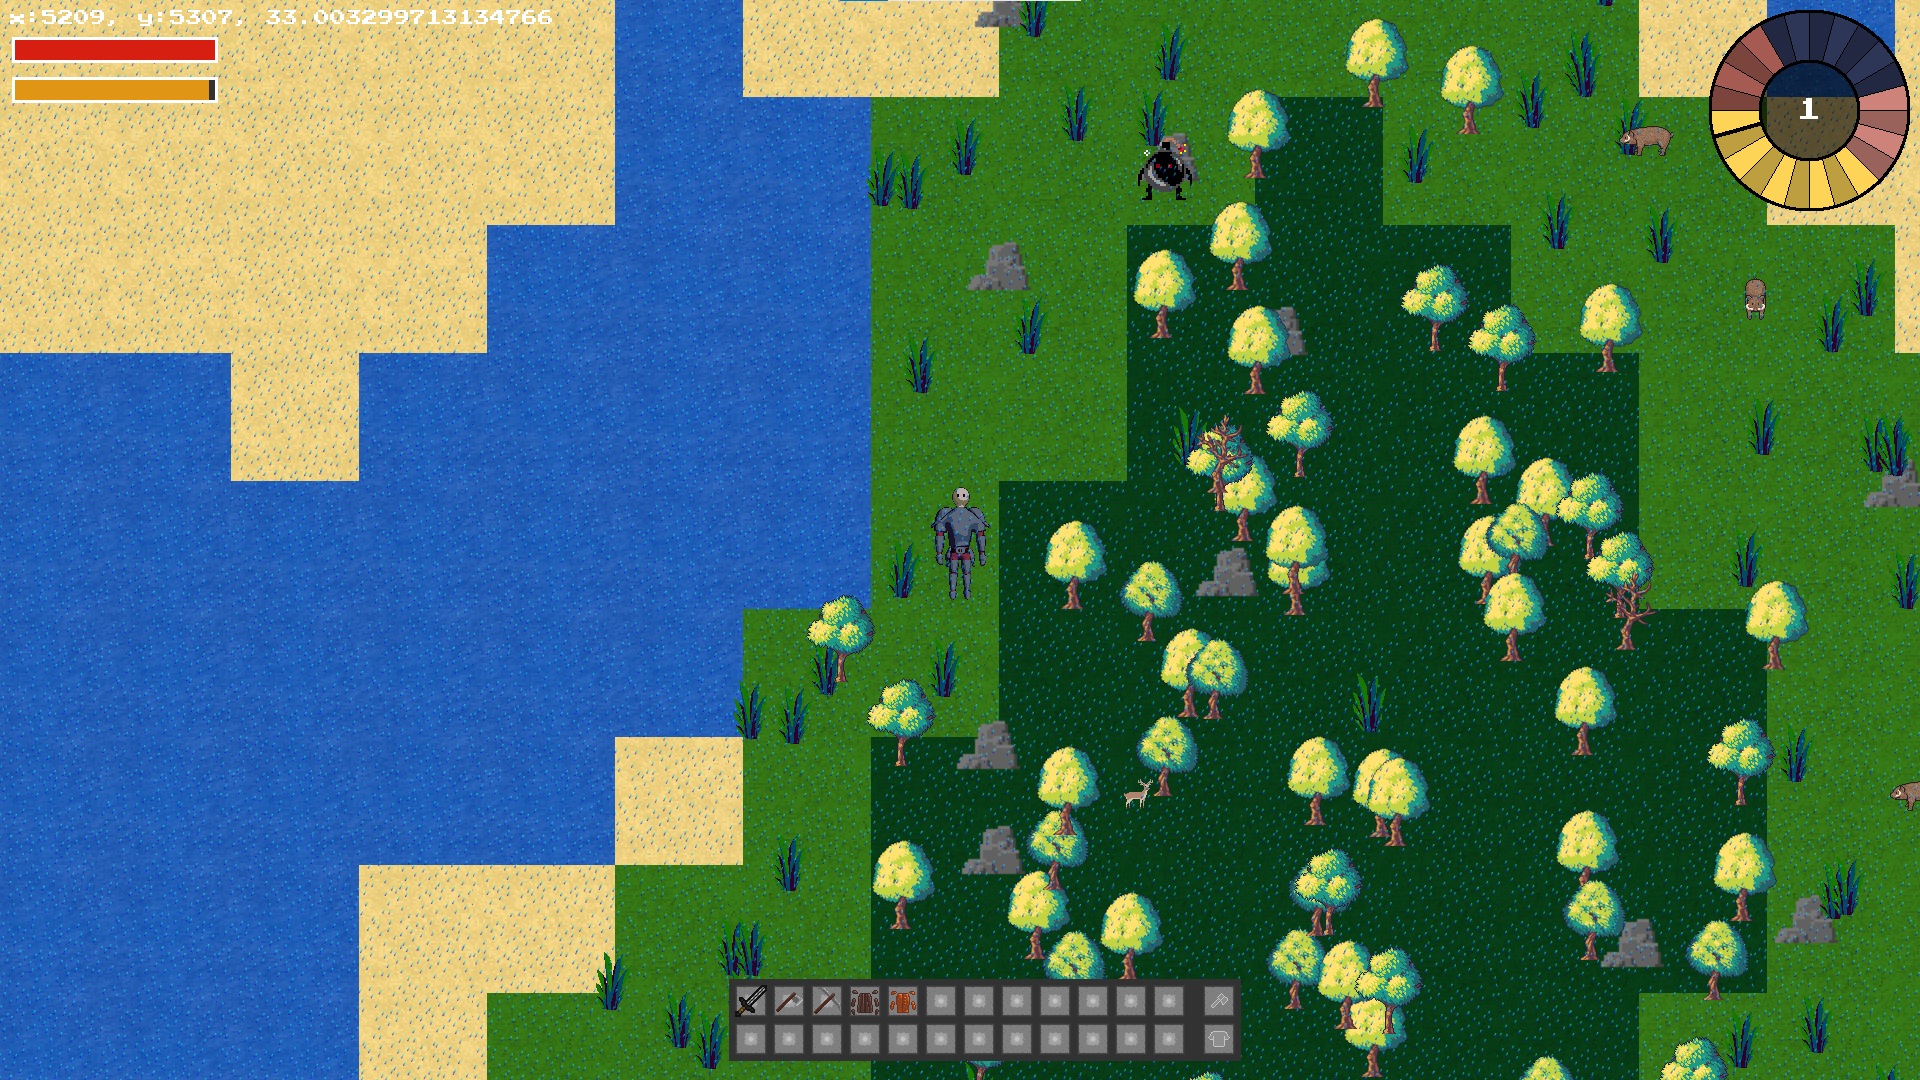
\includegraphics[width=\textwidth]{graDeszcz.png}
     \captionof{figure}{Zrzut ekranu przedstawiający grę podczas deszczu}
\end{center}

\newpage
\section{Implementacja}
\subsection{Architektura rozwiązania}
\subsubsection{Nawigacja w menu}
Architektura gry opiera się na dwóch głównych, zagnieżdżonych pętlach działających do momentu aż użytkownik zdecyduje o ich przerwaniu. Pierwsza z nich, w klasie "MenuController"\space uruchamia się razem z całą aplikacją. W niej poprzez widok menu głównego użytkownik może zdecydować o wyborze zapisu pliku, stworzyć nowy świat, zmienić ustawienia graficzne, głośność dźwięków oraz muzyki.

\begin{center}
    \begin{lstlisting}[language=pythonSchema]
    def menuLoop(self) -> None:
        self.drawMenu()
        while True:
            event = pygame.event.wait()
            self.handleEvent(event)

    def handleEvent(self, event: Event) -> None:
        if event.type == MOUSEMOTION:
            self.drawMenu()
            
        if event.type == MOUSEBUTTONDOWN:
            mousePos = pygame.mouse.get_pos()
            for button in self.currentMenu.buttons:
                if button.checkForInput(mousePos):
                    button.executeAction()

        if event.type == QUIT:
            pygame.quit()
            sys.exit()
            
    def drawMenu(self) -> None:
        self.updateButtons()
        self.screen.blit(self.currentMenu.background, (0, 0))

        for text in self.currentMenu.texts:
            text.draw(self.screen)

        for button in self.currentMenu.buttons:
            button.draw(self.screen)

        pygame.display.update()
    \end{lstlisting}
    \captionof{figure}{Pętla w klasie "MenuController"\space}
\end{center}
\newpage
\subsubsection{Rozpoczęcie rozgrywki}
Gdy użytkownik zdecyduje kliknąć przycisk "PLAY"\space w menu głównym, zostanie przeniesiony do wyboru zapisu. W klasie "MenuController"\space widok zostanie odświeżony za pomocą funkcji "refreshMenu".

\begin{center}
    \begin{lstlisting}[language=pythonSchema]
    def refreshMenu(self) -> None:
        self.currentMenu.reinitializeMenu()
        self.drawMenu()

    def reinitializeMenu(self):
        self.createButtons()
        self.createTexts()
        self.createBackground()

    def drawMenu(self) -> None:
        self.updateButtons()
        self.screen.blit(self.currentMenu.background, (0, 0))

        for text in self.currentMenu.texts:
            text.draw(self.screen)

        for button in self.currentMenu.buttons:
            button.draw(self.screen)

        pygame.display.update()
    \end{lstlisting}
    \captionof{figure}{Funkcja odświeżająca widok menu}
\end{center}

Uruchomienie dowolnego zapisu inicjalizuje klasę "Game".

\begin{center}
    \begin{lstlisting}[language=pythonSchema]
    def createGame(self) -> None:
        mapSize = self.mapSizesList[self.mapSizesIndex]
        objectsQuantity = self.objectsQuantityList[self.objectsQuantityIndex]
        mapRaw, mapData, objects = generateMap(mapSize, objectsQuantity, self.generateMapLoadingScreen)
        saveData = {'map': mapRaw, 'currentDay': 1, 'currentTimeMs': 60000, 'sprites': objects}
        with open(f"savefiles/{self.config.savefileName}.json", "w") as file:
            dump(saveData, file)
        game = Game(self.screen, self.config, saveData)
        game.play()
    \end{lstlisting}
    \captionof{figure}{Inicjalizacja klasy "Game"\space}
\end{center}

Rozpoczęcie rozgrywki wywołuje funkcje zawarte w konstruktorze klasy "Game". W nim na podstawie parametrów zawartych w wybranym pliku, tworzy się interfejs graficzny oraz wszystkie obiekty. Następnie uruchamiana jest pętla główna gry za pomocą instrukcji "game.play()".

\newpage

\begin{center}
    \begin{lstlisting}[language=pythonSchema]
    def play(self) -> None:
        self.changeMusicTheme(HAPPY_THEME)
        while True:
            self.inputManager.handleInput()
            self.dayCycle.updateDayCycle()
            self.visibleSprites.update()
            self.handleTick()
            playerCenter = Vector2(self.player.rect.center)
            self.weatherController.update(playerCenter)
            self.visibleSprites.customDraw(playerCenter)
            self.soundPlayer.currentCameraPos = playerCenter

            self.UiSprites.customDraw()

            text = f"x:{self.player.rect.centerx}, y:{self.player.rect.centery}, {self.clock.get_fps()}"
            self.debug(text)

            pygame.display.update()
            self.clock.tick()
    \end{lstlisting}
    \captionof{figure}{Pętla główna gry}
\end{center}

Od tego momentu w zależności od konkretnych akcji gracza, program zwraca mu odpowiednie rezultaty w formie graficznej, a użytkownik może wchodzić w interakcje z programem zarówno za pomocą myszy jak i klawiatury. Gra się kończy gdy poziom punktów życia gracza spadnie do zera lub gdy uda mu się zniszczyć cztery wieże goblinów. 

\newpage
\subsection{Użyte wzorce projektowe}
\subsubsection{Singleton \cite{wiki:Singleton}}
Singleton jest kreacyjnym wzorcem projektowym, którego celem jest zapewnienie istnienie wyłącznie jednej instancji danej klasy oraz nadanie jej globalnego punktu dostępowego. W niniejszym projekcie przykładem użycia Singletona może być, chociażby klasa "Config"\space przechowująca globalne zmienne czy klasa "Game", w której zawiera się pętla główna gry.
\begin{center}
    \begin{lstlisting}[language=pythonSchema]
class Config:
    def __init__(self) -> None:
        self.monitorWidth = display.Info().current_w
        self.monitorHeight = display.Info().current_h
        self.window = None
        self.WINDOW_WIDTH = self.monitorWidth
        self.WINDOW_HEIGHT = self.monitorHeight
        self.TILES_ON_SCREEN_WIDTH = ceil(self.WINDOW_WIDTH / TILE_SIZE + 1)
        self.TILES_ON_SCREEN_HEIGHT = ceil(self.WINDOW_HEIGHT / TILE_SIZE + 1)
        self.savefileName = None

        # MUSIC
        self.MUSIC_VOLUME = 0.5
        self.SOUNDS_VOLUME = 0.5

        # FONT
        self.FONT = PIXEL_FONT

        self.fontTiny = Font(PIXEL_FONT, FONT_SIZE_TINY)
        self.font = Font(PIXEL_FONT, FONT_SIZE)
        self.fontBig = Font(PIXEL_FONT, FONT_SIZE_BIG)
        self.fontHuge = Font(PIXEL_FONT, FONT_SIZE_HUGE)

    def setFont(self, fontPath: str):
        self.fontTiny = Font(fontPath, FONT_SIZE_TINY)
        self.font = Font(fontPath, FONT_SIZE)
        self.fontBig = Font(fontPath, FONT_SIZE_BIG)
        self.fontHuge = Font(fontPath, FONT_SIZE_HUGE)

    def setWindowSize(self, width: int, height: int):
        self.WINDOW_WIDTH = width
        self.WINDOW_HEIGHT = height
        self.TILES_ON_SCREEN_WIDTH = ceil(self.WINDOW_WIDTH / TILE_SIZE + 1)
        self.TILES_ON_SCREEN_HEIGHT = ceil(self.WINDOW_HEIGHT / TILE_SIZE + 1)
    \end{lstlisting}
    \captionof{figure}{Przykład Singletona: klasa "Config"\space}
\end{center}
\newpage
\subsubsection{Dekorator (ang. Decorator) \cite{wiki:Decorator}}
Dekorator należy do grupy strukturalnych wzorców projektowych. Pozwala on dodawać nowe obowiązki obiektom poprzez umieszczanie ich w specjalnych obiektach opakowujących, które zawierają odpowiednie zachowania. Dotyczy to również funkcji dekorujących, czyli instrukcji, które jako parametr przyjmują funkcje oraz nadają im nowe właściwości. W Pythonie dekoratory oznaczone są znakiem "@"\space i jako parametr przyjmują funkcje bezpośrednio pod nimi.
\begin{center}
    \begin{lstlisting}[language=pythonSchema]
    @state.setter
    def state(self, newState: State) -> None:
        if newState == State.DAMAGED:
            self.__changeImages(self.imageUpDamage, self.imageDownDamage, self.imageLeftDamage, self.imageRightDamage)
        elif newState == State.HEALED:
            self.__changeImages(self.imageUpHeal, self.imageDownHeal, self.imageLeftHeal, self.imageRightHeal)
        else:
            self.__changeImages(self.imageUpNormal, self.imageDownNormal, self.imageLeftNormal, self.imageRightNormal)
        self._state = newState
    \end{lstlisting}
    \captionof{figure}{Przykład użycia funkcji dekorującej w projekcie state.setter}
\end{center}
\subsubsection{Stan (ang. State) \cite{wiki:State}}
Stan to behawioralny wzorzec projektowy, który umożliwia obiektowi modyfikację swojego zachowania poprzez zmianę stanu wewnętrznego. W niniejszym projekcie przykład użycia tego wzorca znajduje się w klasie "Entity".
\begin{center}
    \begin{lstlisting}[language=pythonSchema]
    @state.setter
    def state(self, newState: State) -> None:
        if newState == State.DAMAGED:
            self.__changeImages(self.imageUpDamage, self.imageDownDamage, self.imageLeftDamage, self.imageRightDamage)
        elif newState == State.HEALED:
            self.__changeImages(self.imageUpHeal, self.imageDownHeal, self.imageLeftHeal, self.imageRightHeal)
        else:
            self.__changeImages(self.imageUpNormal, self.imageDownNormal, self.imageLeftNormal, self.imageRightNormal)
        self._state = newState
    \end{lstlisting}
    \captionof{figure}{Przykład zarządzania stanem klasy "Entity"\space z użyciem dekoratora state.setter}
\end{center}
\newpage
\subsubsection{Fabryka (ang. Factory) \cite{wiki:Factory}}
W trakcie, gdy gra działa spora część operacji to tworzenie nowych obiektów, stąd fabryka jest wyjątkowo pasującym wzorcem projektowym. Jego głównym założeniem, tak jak w rzeczywistym świecie, jest wytwarzanie obiektów. Dzięki wykorzystaniu fabryki można ukryć szczegóły implementacyjne tworzenia obiektów i odseparować je od logiki biznesowej. Jedną z fabryk w niniejszym projekcie jest "GoblinFactory".
\begin{center}
    \begin{lstlisting}[language=pythonSchema]
class GoblinFactory:
    def __init__(self, visibleSprites: CameraSpriteGroup, obstacleSprites: ObstacleSprites,
                 loadedImages: LoadedImages, loadedSounds: LoadedSounds,
                 clock: Clock, soundPlayer: SoundPlayer):
        self.visibleSprites = visibleSprites
        self.loadedImages = loadedImages
        self.loadedSounds = loadedSounds
        self.obstacleSprites = obstacleSprites
        self.clock = clock
        self.soundPlayer = soundPlayer

    def createGoblin(self, pos, currHealth: int | None = None) -> Goblin:
        newGoblin = Goblin(self.visibleSprites, self.obstacleSprites, self.loadedImages, self.loadedSounds, self.clock,
                           pos, self.soundPlayer, currHealth)
        return newGoblin

    def createGoblinChampion(self, pos, currHealth: int | None = None) -> GoblinChampion:
        newGoblinChampion = GoblinChampion(self.visibleSprites, self.obstacleSprites, self.loadedImages,
                                           self.loadedSounds, self.clock, pos, self.soundPlayer, currHealth)
        return newGoblinChampion
    \end{lstlisting}
    \captionof{figure}{Przykład factory: klasa "GoblinFactory"\space}
\end{center}
\newpage
\subsubsection{Obserwator (ang. Observer) \cite{wiki:Observer}}
Obserwator to czynnościowy (behawioralny) wzorzec projektowy pozwalający zdefiniować mechanizm subskrypcji w celu powiadamiania zainteresowanych obiektów o zmianie stanu innego obiektu.
\begin{center}
    \begin{lstlisting}[language=pythonSchema]
class DayPhaseListener:
    def onDay(self):
        pass

    def onEvening(self):
        pass

    def onMorning(self):
        pass

    def onNight(self):
        pass

class DayPhaseEventManager:
    def __init__(self):
        self.listeners: dict[DayPhase, list[DayPhaseListener]] = {}
        self.dayPhasesNotifiers: dict[DayPhase, Callable[[DayPhaseListener], None]] = {
            DayPhase.DAY: (lambda listener: listener.onDay()),
            DayPhase.NIGHT: (lambda listener: listener.onNight()),
            DayPhase.MORNING: (lambda listener: listener.onMorning()),
            DayPhase.EVENING: (lambda listener: listener.onEvening())
        }

    def subscribe(self, dayPhaseEvent: DayPhase, listener: DayPhaseListener):
        eventListeners = self.listeners.get(dayPhaseEvent, [])
        eventListeners.append(listener)
        self.listeners[dayPhaseEvent] = eventListeners

    def unsubscribe(self, dayPhaseEvent: DayPhase, listener: DayPhaseListener):
        self.listeners[dayPhaseEvent].remove(listener)

    def notify(self, dayPhaseEvent: DayPhase):
        for listener in self.listeners.get(dayPhaseEvent, []):
            self.dayPhasesNotifiers[dayPhaseEvent](listener)

    \end{lstlisting}
    \captionof{figure}{Przykład obserwatora: klasy "DayPhaseListener"\space i "DayPhaseEventManager"\space}
\end{center}
\subsection{Diagram uwzględniający architekturę całości}
Cała architektura gry bazuje na kilku pętlach. W trakcie działania aplikacji w zależności od ścieżki w menu, którą wybierze gracz poszczególne moduły uruchamiają swoje własne pętle. Poniższy diagram przedstawia zależności pomiędzy nimi.
\begin{center}
     \includegraphics[width=\textwidth]{architektura_rozwiazania.png}
     \captionof{figure}{Diagram architektury całości}
\end{center}
\subsection{Użyte technologie}
\subsubsection{Python \cite{tech:Python}}
Jedynym językiem programowania użytym w niniejszej pracy jest wysokopoziomowy język Python. Umożliwia programowanie obiektowe i funkcyjne, a charakteryzuje go prosta oraz przejrzysta składnia.
\subsubsection{Pygame \cite{tech:Pygame}}
Pygame jest biblioteką w języku Python, która dostarcza niezbędnych narzędzi do tworzenia gier oraz aplikacji multimedialnych z wykorzystaniem grafiki, dźwięku i animacji. Jest to główna technologia, na której bazuje niniejsza gra.
\subsubsection{NumPy \cite{tech:NumPy}}
NumPy jest bardzo popularną biblioteką do obliczeń naukowych, która dostarcza funkcje ułatwiające pracę z wielowymiarowymi tablicami i macierzami.
\section{Testy}
\subsection{Testy manualne}
\subsubsection{Wstęp}
Testy manualne są nieodłącznym elementem wysokiej jakości oprogramowania. Pozwala nie tylko wykryć bardziej skomplikowane błędy, które ciężko wykryć przy pomocy testów jednostkowych, ale również zmierzyć cechy takie jak satysfakcja z rozgrywki lub poziom trudności. Dwie ostatnie rzeczy są niemożliwe do sprawdzenia przy pomocy kodu, dlatego przyłożyliśmy dużą wagę do tego rodzaju testów w naszym projekcie.
\subsubsection{Przykładowy scenariusz testowy}
\textbf{ID:} FSE-04 \\
\textbf{Tytuł:} Test interakcji gracza z przedmiotami \\
\textbf{Warunki wstępne:} \\
- Stworzona gra ze światem o dowolnym rozmiarze \\
- Gracz posiada przedmiot w ekwipunku \\
\textbf{Kroki testowe:} \\
\begin{center}
\begin{tabularx}{\textwidth} {
| >{\centering\arraybackslash}p{0.02\textwidth}
| >{\centering\arraybackslash}X
| >{\centering\arraybackslash}X | }
\hline
Nr. & Krok & Oczekiwany rezultat \\
\hline
\begin{center}
1.
\end{center} &
\begin{center}
Gracz klika na przedmiot znajdujący się w ekwipunku
\end{center}
&
\begin{itemize}
\item Przedmiot znika z ekwipunku
\item Przedmiot łączy się do kursora myszki
\end{itemize} \\
\hline
2. & Gracz przesuwa kursor myszki & Przedmiot podąża za kursorem myszki \\
\hline
\begin{center}
3.
\end{center} &
\begin{center}
Gracz naciska lewy przycisk myszki na dowolny pusty obszar na mapie
\end{center}
&
\begin{itemize}
\item Postać podchodzi do wyznaczonego miejsca
\item Przedmiot pojawia się w świecie gry
\item Przedmiot odłącza się od kursora myszki
\end{itemize} \\
\hline
4. & Gracz wciska dowolny klawisz ruchu & Gracz znajduje się w widocznej odległości od przedmiotu \\
\hline
5. & Gracz najeżdża kursorem myszki na przedmiot widoczny na mapie & Kursor gracza znajduje się nad przedmiotem \\
\hline
6. & Gracz wciska lewy przycisk myszki & Przedmiot pojawia się w pierwszym wolnym gnieździe w ekwipunku \\
\hline
\end{tabularx}
\end{center}

Powyższy przypadek testowy sprawdza, czy gra umożliwia podnoszenie i wyrzucanie przedmiotów. Określa sposób wizualizacji oraz zachowania postaci, dzięki czemu możemy sprawdzać wiele parametrów za jednym razem.
\subsection{Testy integracyjne}
\subsubsection{Wstęp}
Testy integracyjne są kolejnym elementem piramidy testów. Ich zadaniem jest sprawdzenie współdziałania całego systemu lub jego części. Pozwalają między innymi wykryć problemy z nieprawidłowym przepływem danych, komunikacją pomiędzy modułami oraz zależnościami. W przypadku naszego projektu testy integracyjne są kluczowym etapem w procesie weryfikacji poprawności działania wszystkich składników gry. Pozwalają upewnić się, że cały system działa zgodnie z oczekiwaniami i spełnia założone wymagania.
\subsubsection{Testowanie komunikacji między modułami}
Możliwość kontrolowania bohatera przez gracza, jest jedną z podstawowych mechanik w naszym projekcie. By przetestować tę funkcjonalność, wykonujemy testy integracyjne sprawdzające komunikację między modułem odpowiedzialnym za wykrywanie wciśniętych klawiszy przez użytkownika, a modułem zarządzającym przemieszczaniem postaci.

\begin{lstlisting}[language=pythonSchema]
def test_player_should_move_forward_when_user_press_w(self):
    pygame.key.get_pressed = (lambda: {K_w: True, K_s: False, K_a: False, K_d: False})

    self.inputManager.handleInput()
    self.player.update()

    self.assertEqual(self.player.rect.midbottom, (self.playerPosBeforeMove.x, self.playerPosBeforeMove.y - 6))

def test_player_should_move_left_when_user_press_a(self):
    pygame.key.get_pressed = (lambda: {K_w: False, K_s: False, K_a: True, K_d: False})

    self.inputManager.handleInput()
    self.player.update()

    self.assertEqual(self.player.rect.midbottom, (self.playerPosBeforeMove.x - 6, self.playerPosBeforeMove.y))
\end{lstlisting}
Powyżej zostały przedstawione dwa przykładowe testy sprawdzające tę funkcjonalność. Każdy z testów składa się z trzech sekcji: Arrange, Act i Assert\cite{tech:ArrangeActAssert}, dzięki czemu są dobrze ustrukturyzowane oraz łatwo można je przeczytać.

W pierwszej sekcji przygotowujemy dane niezbędne do wykonania tej operacji. Modyfikujemy funkcję "get\_pressed"\space z biblioteki Pygame, która zwraca słownik, gdzie kluczem jest przycisk, a wartością jest informacja o tym, czy został wciśnięty.

Następnie wywołujemy funkcję odpowiedzialną za sczytywanie wciśniętych klawiszy oraz funkcję odpowiedzialną za zaktualizowanie postaci gracza.

Na koniec sprawdzamy, czy pozycja gracza zmieniła się zgodnie z naszymi oczekiwaniami.
\subsubsection{Testowanie mechanik gry}
Gra składa się z wielu różnych mechanik, które wpływają na siebie nawzajem. Dzięki testom integracyjnym mamy możliwość sprawdzenia, czy wszystkie mechaniki współpracują ze sobą, tak jak przewidzieliśmy.

Poniższy fragment kodu ma na celu sprawdzenie, czy założenie przez gracza zbroi wpływa na otrzymywane przez niego obrażenia:
\begin{lstlisting}[language=pythonSchema]
def test_player_should_get_lower_damage_when_armor_is_equipped(self):
    self.player.bodySlot.item = self.leatherArmor

    self.player.getDamage(10)

    self.assertEqual(self.player.currHealth, self.playerHealth - 6)
\end{lstlisting}

Kolejnym przykładem zastosowania testów integracyjnych do testowania zależności między mechanikami jest sprawdzanie, czy gracz będzie zadawał większe obrażenia po wyposażeniu w broń.
\begin{lstlisting}[language=pythonSchema]
def test_player_should_deal_higher_damage_when_weapon_is_equipped(self):
    self.player.handSlot.item = self.weapon

    damageDealt = self.player.damage()

    self.assertEqual(damageDealt, 10)
\end{lstlisting}
Na powyższym teście testujemy czy obrażenia zadawane przez gracza wzrosły do dziesięciu punktów życia z bazowych trzech punktów po umieszczeniu miecza w odpowiednim gnieździe ekwipunku.
\subsection{Testy jednostkowe}
\subsubsection{Wstęp}
Ciężko wyobrazić sobie rozwój jakiejkolwiek aplikacji bez podstawy piramidy testów. Testy jednostkowe służą weryfikacji poprawności działania pojedynczych elementów programu - np. metod lub obiektów i składają się z jednej asercji.

\subsubsection{Przykładowe scenariusze testowe}
Testy jednostkowe mogą sprawdzać bardzo wiele parametrów. Przykładami mogą być testy weryfikujące poprawność nazwy przedmiotu.

\begin{center}
    \begin{lstlisting}[language=pythonSchema]
def test_item_name_initializes(self):
    self.assertEqual(self.item.name, "Leather")
    \end{lstlisting}
    \captionof{figure}{Przykład testu jednostkowego dla klasy Item}
\end{center}

Za pomocą tego typu testów można też sprawdzać czy dany parametr nie jest równy pewnej wartości, czego przykładem może być weryfikacja unikalności id przedmiotu.

\begin{center}
    \begin{lstlisting}[language=pythonSchema]
self.item = Item(self.visibleSprites, Vector2(0, 0), self.loadedImages)
self.item2 = Item(self.visibleSprites, Vector2(0, 0), self.loadedImages)

def test_id_should_be_different_between_items(self):
    self.assertNotEqual(self.item.id, self.item2.id)
    \end{lstlisting}
    \captionof{figure}{Przykład testu jednostkowego dla klasy Item}
\end{center}

Kolejną funkcją dostarczaną przez pytest jest możliwość weryfikacji czy dane zawierają się w tablicy.

\begin{center}
    \begin{lstlisting}[language=pythonSchema]
def test_drop_should_add_item_to_visibleSprites(self):
    self.item.drop(Vector2(0, 0))
    self.assertIn(self.item, self.visibleSprites)
    \end{lstlisting}
    \captionof{figure}{Przykład testu jednostkowego dla klasy Item}
\end{center}

Jednak możliwości testów jednostkowych nie ograniczają się na weryfikacji prawdziwości parametrów obiektu. Przykładem może być asercja weryfikująca liczbę wywołań danej funkcji.

\begin{center}
    \begin{lstlisting}[language=pythonSchema]
def test_onLeftClickAction_should_call_inventory_addItem(self):
    self.item.onLeftClickAction(self.player)
    self.player.inventory.addItem.assert_called_once()
    \end{lstlisting}
    \captionof{figure}{Przykład testu jednostkowego dla klasy Innventory}
\end{center}

\subsection{Testy wydajnościowe}
\subsubsection{Wstęp}
Podczas tworzenia aplikacji szczególną uwagę przykładaliśmy do jej optymalizacji. Dzięki licznym zmianom i usprawnieniom działania poszczególnych klas gra przy domyślnych ustawieniach działa w ponad 40 FPS'ach, które stanowiły docelowy próg. Poniżej opiszemy szczególnie ciekawe przypadki optymalizacyjne.
\subsubsection{Konwersja formatu pikseli}
W początkowym etapie rozwoju aplikacji natknęliśmy się na problem z wyświetlaniem elementów na ekranie. Polegał on na tym, że czas potrzebny na wyświetlenie wszystkich widzialnych sprite'ów, których było na tym etapie niewiele, zajmowało zbyt wiele czasu, aby można było skutecznie zwiększyć ich liczbę, poprzez zagęszczenie ich, bądź zwiększenia rozdzielczości okna aplikacji.

Podczas prób rozwiązania tego problemu testowaliśmy takie rozwiązania jak łączenie fragmentów mapy w większe kawałki, aby zmniejszyć liczbę wywołań funkcji "blit", która jest częścią biblioteki Pygame, lecz to nie rozwiązało problemu, co pozwoliło nam zrozumieć, że liczba wywołań tej funkcji nie jest przyczyną.

Po dogłębnej analizie odkryliśmy, że po załadowaniu obrazu z pamięci komputera przy pomocy funkcji "load", będącą częścią biblioteki Pygame, owa grafika zachowywała swój format pikselowy\cite{wiki:pix}, czyli format w jaki przechowywane są informacje o pojedynczym pikselu obrazu. Z tego powodu funkcja "blit"\space za każdym wywołaniem musiała najpierw zmienić format pikselowy obrazu, który zapisany był na 32 bitach, aby ten odpowiadał domyślnemu formatowi zapisanemu na 8 bitach.

Rozwiązaniem była konwersja formatu pikselowego wszystkich grafik tuż po załadowaniu ich z pamięci. Ten problem dał początek klasie "LodedImages", która zajmuje się ładowaniem i konwersją wszystkich obrazów, dzięki czemu wszystkie grafiki przechowywane są w jednym miejscu i nie ma potrzeby ich wielokrotnego ładowania.

\subsubsection{Detekcja kolizji}
Innym problemem optymalizacyjnym, na jaki napotkaliśmy podczas tworzenia aplikacji było efektywne wykrywanie kolizji. Detekcja kolizji zajmuje znaczną część zasobów procesora i jest jednym z bardziej wymagających zagadnień pod względem implementacyjnym.

Jedną z jej części jest znajdywanie zbioru obszarów blokujących ruch. W naszej grze obszary wywołujące kolizje są określone wyłącznie przez instancje klasy "CollisionObject"\space i fragmenty mapy stanowiące morze. W pierwszych wersjach gry stwory sprawdzały wszystkie te obszary podczas detekcji kolizji, co przy niewielkim rozmiarze mapy i braku obiektów klasy "CollisionObject"\space nie stanowiło problemu.

Po zaimplementowaniu nowego sposobu generacji mapy wielkość morza znacznie się zwiększyła, co sprawiło, że nawet przy braku obiektów klasy "CollisionObject"\space ilość czasu potrzebnego na detekcję kolizji była zbyt duża. Rozwiązaniem było napisanie funkcji, która zwracała listę tylko tych fragmentów morza, z którym dany stwór bezpośrednio graniczy, co sprawiło, że na tamten moment liczba obszarów kolizji do sprawdzenia zmniejszyła się z kilku tysięcy do liczby z przedziału od 0 do 7. Ta zmiana sprawiła, że czas potrzebny na wykrywanie kolizji stał się krótszy niż przed wprowadzeniem nowego sposobu generacji mapy.

Po zaimplementowaniu klasy "CollisionObject"\space korzystając z wcześniejszych doświadczeń postanowiliśmy, że ograniczymy również ilość nowopowstałych obszarów kolizji do sprawdzania poprzez sprawdzanie tylko tych, które znajdują się w niedalekiej odległości od stwora. Niestety okazało się, że funkcja "colliderect", będąca częścią biblioteki Pygame, z której korzystaliśmy, aby wykryć kolizję, ma już w sobie wbudowane takowe systemy, a nasza próba przyniosła odwrotne rezultaty, więc powróciliśmy do sprawdzania wszystkich obszarów kolizji wyznaczanych przez "CollisionObject".

Poniżej znajduje się wykres porównujący efektywność wszystkich testowanych przez nas sposobów ograniczania ilości obszarów kolizji do sprawdzenia, gdzie rozmiar próby oznacza ilość obiektów blokujących ruch i stworów, ilość fragmentów morza wynosiła kolejno 36 i 76, a sposoby przedstawione na wykresie odpowiadają tym opisanym w poniższej tabeli.

\begin{center}
 \begin{tabularx}{\textwidth} { 
  | >{\centering\arraybackslash}p{0.14\textwidth} 
  | >{\centering\arraybackslash}X 
  | >{\centering\arraybackslash}X | }
 \hline
  Nr. sposobu & fragmenty morza & "CollisionObject"\space \\
 \hline
 1 & wyłącznie graniczące ze stworem & wyłącznie w pobliżu stwora \\
 \hline
 2 & wyłącznie graniczące ze stworem & wszystkie \\
 \hline
 3 & wszystkie & wszystkie \\
 \hline
 \end{tabularx}
\end{center}

\begin{center}
     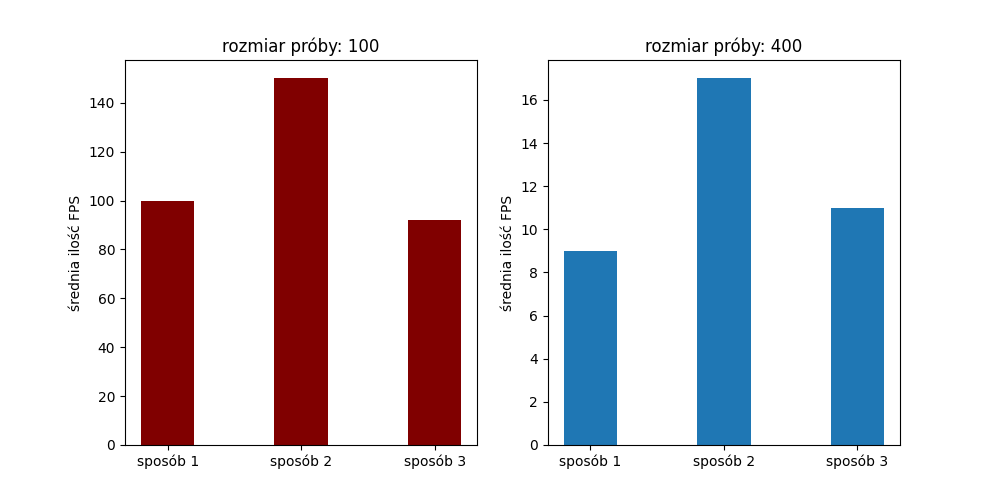
\includegraphics[width=\textwidth]{collisionPlot.png}
     \captionof{figure}{Wykres porównujący efektywność sposobów ograniczania ilości obszarów kolizji do sprawdzenia}
\end{center}

\subsubsection{Efekt ciemności}
Dzień w świecie naszej gry składa się z czterech faz kolejno: poranka, dnia, wieczoru i nocy. Wszystkie te fazy wpływają na rozgrywkę poprzez ograniczanie widoczności gracza za sprawą maski nakładanej na obraz.

Podczas dnia widoczność gracza nie jest w żaden sposób ograniczona, gdy nastaje wieczór wszystko poza zasięgiem światła, które jest emitowane za sprawą instancji klasy "Glowing", staje się coraz ciemniejsze, aż do momentu, gdy staje się całkowicie czarne, co jest równoznaczne z nastaniem nocy.

Podczas poranku odwrotnie do wieczoru wszystko znów staje się widoczne. Pierwotnie udało się nam osiągnąć ten efekt wyrysowywując na ekranie (na którym wszystkie elementy świata były już wyrysowane, a interfejs użytkownika jeszcze nie) czarną maskę\footnote{maska w znaczeniu warstwy nakładanej na obraz w celu osiągnięcia zamierzonego efektu artystycznego.}.

Efekt płynnego przejścia pomiędzy dniem a nocą działał na podstawie zmieniania przezroczystości owej maski, a wpływ światła na nią był symulowany za pomocą wyrysowywania na niej obrazu światła (który był czarno-przezroczysty) za pomocą wbudowanej w bibliotekę Pygame funkcji "blit", z użyciem specjalnej flagi "BLEND\_RGBA\_SUB", która sprawiała, że wartości pojedynczych pikseli zamiast być dodawane, były od siebie odejmowane, przez co obszar, na którym wyrysowywane było światło stawał się półprzezroczysty. Mimo że to rozwiązanie pozwoliło nam osiągnąć zamierzony efekt, tak liczna ilość półprzezroczystych pikseli do wyrysowania zbytnio obciążała procesor, przez co ilość FPS podczas poranków i wieczorów była zbyt niska.

Po licznych próbach optymalizacji tej funkcjonalności doszliśmy do wniosku, że musimy znacznie ograniczyć ilość operacji związanych z wyrysowywaniem półprzezroczystych pikseli. Zaczęliśmy od zmiany podejścia w jaki osiągamy efekt płynnego przejścia z dnia do nocy, poprzez całkowite usunięcie przezroczystości maski na rzecz zastąpienia czarnego koloru jego odcieniem, a wyrysowywanie grafik światła (które od teraz były biało-przezroczyste) korzystało z podstawowej wersji funkcji "blit", bez specjalnych flag.

Ta zmiana spowodowała też, że sposób w jaki owa maska była wyrysowywana na ekranie również musiał ulec zmianie i od tej pory zamiast używania funkcji "blit"\space w domyślnej konfiguracji, korzystaliśmy z niej z użyciem specjalnej flagi "BLEND\_RGBA\_MULT", która sprawiała, że wartości pikseli zamiast być do siebie dodawane, tak jak jest w domyślnej wersji, były przez siebie wymnażane. Dzięki tej zmianie udało się nam uniknąć znacznej ilości operacji związanych z przezroczystością pikseli, dzięki czemu ogólna rozgrywka stała się znacznie płynniejsza niezależnie od pory dnia.

\subsection{Podsumowanie}
Dzięki przeprowadzonym różnym rodzajom testów, mamy pewność, że nasza gra jest w pełni działająca, spełnia początkowe oczekiwania i jest wolna od wszelkich defektów. Jest to zasługą wielu iteracji naszej bazy testów oraz wkładu całego zespołu pracującego nad projektem, który czuwał nad jakością implementowanych funkcjonalności. Jesteśmy zadowoleni z ośiągnietego rezultatu i mamy nadzieje że nasza gra dostarczy niezapomnianą rozrywkę swoim przyszłym graczom.
\section{Podział prac w projekcie}
\subsection{Paweł Olszewski}
\subsubsection{Zarządzanie}
Jako leader zespołu Paweł był odpowiedzialny za organizowanie cotygodniowych spotkań, na których przydzielał wszystkim członkom zespołu zadania i pomagał rozwiązywać problemy, na które napotkali. Poza tym czuwał nad jakością kodu poprzez dokonywanie inspekcji kodu\cite{wiki:inspekcja} i wprowadzania usprawnień za każdym razem, gdy funkcjonalność rozwijana przez jednego z członków zespołu była ukończona.
% Przypadkami usprawnień kodu które były najistotniejsze to optymalizacja sposobu działania menu oraz optymalizacja działania mechaniki faz dnia.

\subsubsection{Działanie gry}
Głównym zadaniem Pawła było definiowanie podstawowego działania mechanik gry, takich jak wyświetlanie grafik na ekranie, wczytywanie grafik, reagowanie na akcje użytkownika, w tym interakcje z obiektami, stworami i przedmiotami, dodanie pór roku, czy ekran wczytywania oraz zakończenie gry.
% - ui i camera sprite group\\
% - inputManager (reakcja na input użytkownika)\\
% - ekran końca gry\\

\subsubsection{Generator świata gry}
Zajmował się również tworzeniem generatora świata gry, w skład którego wchodzi proceduralne generowanie mapy świata oraz znajdujących się na niej obiektów i stworów. Dodatkowo mapa świata jest podzielona na biomy, które różnią się obiektami i stworami, które się na nich generują, a fragmenty lądu graniczące z morzem korzystają ze zmodyfikowanych grafik.

\subsubsection{Stwory}
Zadaniem Pawła było również stworzenie klasy "Entity", po której dziedziczą wszystkie stwory w grze, a która kontroluje takie aspekty jak poruszanie się czy detekcję kolizji. Dodatkowo był odpowiedzialny za klasę "Player", której instancja stanowi postać gracza.

\subsubsection{Usprawnienia oraz optymalizacja istniejących funkcjonalności}
Znaczna część prac Pawła poza tworzeniem nowych mechanik polegała na usprawnianiu istniejących, oraz rozszerzaniu ich o nowe funkcjonalności. Przypadkami usprawnień kodu które były najistotniejsze to optymalizacja sposobu działania menu, optymalizacja działania mechaniki faz dnia, w tym stworzenie zegara stanowiącego część interfejsu użytkownika, dodanie animowanych obiektów oraz dodanie specjalnych pól w ekwipunku na narzędzia i zbroje, wraz ze związanymi z nimi mechanikami .

\subsubsection{Stan gry}
Jedną z bardziej złożonych funkcjonalności stworzonych przez Pawła było zapisywanie i wczytywanie stanu gry, wraz z odpowiednim widokiem w menu.

\subsubsection{Tworzenie dokumentacji}
Z części opisowej tej pracy Paweł odpowiadał za napisanie rozdziału 2 - Projekt i analiza, podrozdziału 4.4 - Testy Wydajnościowe, oraz tej części rozdziału piątego.

%  Był również odpowiedizalny za poprawne działanie postaci którą gracz kontroluje, która jest instancją klasy "Player", przechowującą wszystkie informacje o postaci gracza, wraz z niezbędną logiką. 
% "InputManager", która reaguje na akcje użytkownika

\subsection{Kacper Krüger}
\subsubsection{Ekwipunek}
Jednym z pierwszych zadań Kacpra odnośnie projektu, było zaimplementowanie ekwipunku, w którym gracz mógłby trzymać zdobyte przedmioty podczas rozgrywki. Z tym problemem pomógł mu Paweł Olszewski, który zaprojektował oryginalny interfejs graficzny dopasowany do naszej gry, oraz wprowadził drobne zmiany w kodzie w celu zwiększenia czytelności.
\subsubsection{Obiekty}
Kacper zajmował się również stworzeniem klasy abstrakcyjnej "Object", która jest bazą dla wszystkich obiektów w naszym projekcie. Jednocześnie zaimplementował kilka obiektów rozszerzających tę klasę, takich jak kamień, pierwszą wersję trawy, króliczą norę, oraz wszystkie rodzaje drzew wraz z ich cyklem życia.
\subsubsection{Przedmioty}
W ramach projektu Kacper opracował również pierwszą wersję klasy "Item", która implementuje wszystkie przedmioty w naszej grze. Klasa zawierała podstawowe informacje o przedmiocie oraz umożliwiała trzymanie ich w ekwipunku, oraz pozostawienie na mapie. Ta klasa została mocno rozwinięta w późniejszych etapach rozwoju projektu przez Pawła Olszewskiego.
\subsubsection{Świecące obiekty i stwory}
Kolejnym jego zadaniem było dodanie do systemu dnia i nocy źródeł światła. Ten problem zapoczątkował klasę "Glowing", która pozwala wybrać wielkość jak i dokładnie określić miejsce z którego światlo będzie się wydobywać. Tą klasę mogą implementować zarówno stwory jak i przedmioty. Jednak wraz z dodawaniem większej ilości świecących obiektów, natknęliśmy się na problem z optymalizacją jego rozwiązania, który rozwiązał i opisał w dziale testy wydajnościowe Paweł Olszewski. 
\subsubsection{Stwory}
Należało do niego rozszerzenie abstrakcyjnej klasy "Entity"\space poprzez stworzenie kolejnych abstrakcyjnych klas: "AgresiveMob", "NeutralMob"\space i "FriendlyMob", które określają zachowania w wobec gracza oraz innych stworów dla danej klasy. Stworzył również: jelenia, dzika oraz królika, które implementują wcześniej wymienione klasy.
\subsubsection{Testy}
Jednym z jego zadań było stworzenie scenariuszy do testów manualnych, testów integracyjnych oraz części testów jednostkowych.
\subsubsection{Tworzenie dokumentacji}
W jego przypadku głównym elementem merytorycznym tej pracy był rozdział pierwszy. Napisałem również część rozdziału czwartego dotyczącą testów manualnych, integracyjnych oraz ten podrozdział pracy.

\subsection{Maksymilian Keller}
\subsubsection{Muzyka}
Maksymilian napisał, nagrał i dołączył do aplikacji autorską muzykę. W zależności od tego czy gracz jest w menu, czy w trakcie rozgrywki towarzyszy mu unikalna melodia, której głośność można zmienić w menu. Dodanie obsługi muzyki umożliwiło również dołączanie dźwięków do rozgrywki innym uczestnikom projektu.

\subsubsection{Menu}
Głównym elementem prac merytorycznych Maksymiliana było zaprojektowanie Menu gry zarówno od strony graficznej jak i technicznej. Między innymi dodał możliwości zmiany głośności muzyki, dźwięków, czcionki i rozdzielczości oraz zaprojektował i wdrożył system przechodzenia pomiędzy poszczególnymi widokami w Menu.

\subsubsection{Namiot}
Ciekawym urozmaiceniem rozgrywki jest możliwość spędzenia nocy w namiocie. Jest to specjalny obiekt na mapie, który w określonych porach umożliwa graczowi pominięcie godzin wieczornych.

\subsubsection{GoblinWatchTower - wieża goblinów}
Prawdopodobnie najistotniejszym pod względem ogółu rozgrywki zadaniem Maksymiliana było dodanie mechaniki GoblinWatchTower. Jest ona zaimplementowana w ten sposób, że po zniszczeniu czterech wież strzeżonych przez kilku automatycznie generowanych strażników gracz wygrywa grę. W przypadku gdy użytkownik wejdzie na teren wieży, atakują go gobliny, a gdy wyjdzie poza jej zasięg, wartownicy automatycznie wracają do swojego schronienia. Liczba zniszczonych wież oraz strażników podlega zapisowi, a gobliny po czasie mogą pojawić się ponownie na mapie.

\subsubsection{Refactor i testy}
Kilka mniejszych zadań Maksymiliana skupiało się na ulepszeniu obecnych rozwiązań pod względem czytelności kodu oraz dopisaniu testów (głównie jednostkowych).

\subsubsection{Tworzenie dokumentacji}
Podobnie jak prawie każdy z autorów, Maksymilian odpowiadał za napisanie części tej pracy. W tym przypadku był to rozdział trzeci, część rozdziału czwartego dotycząca testów jednostkowych oraz ta subsekcja na temat podziału pracy.

\subsection{Mateusz Maćkowiak}
\subsubsection{Animowane stwory}
Klasa "AnimatedEntity"\space stworzona przez Mateusza na podstawie klasy "AnimatedObject", stworzonej przez Pawła pozwalająca na wyświetlanie różnych animacji w zależności od stanu, w którym się znajdował stwór. Przykładem takiego potwora jest klasa "GoblinChampion".

\subsubsection{Gobliny}
Mateusz stworzył klasę "Goblin", która odpowiada za zachowanie najliczniej występującego przeciwnika. Goblin nie atakuje innych goblinów, a po śmierci wypada z niego przedmiot "GoblinFang". Rozszerzeniem tej klasy jest "GoblinChampion". Posiada on animacje bezruchu, chodzenia i atakowania w czterech kierunkach. Kryjówka Goblinów, klasa "GoblinHideout", tworzy nowe gobliny, jeżeli ich liczba spadnie poniżej pewnej wartości.  

\subsubsection{Cykl dnia i nocy}
Mateusz zaimplementował wczesną wersję cyklu faz dnia. Prototyp tworzył półprzezroczystą maskę nakładaną na obraz w celu osiągnięcia wizualnego efektu ciemności. To rozwiązanie zostało następnie rozwinięte przez Pawła Olszewskiego w celu zwiększenia liczby FPS.

\subsubsection{Skrypty pomocnicze}
Mateusz zaprojektował skrypt "RescaleGraphics"\space zmieniający rozmiar grafik oraz skrypt "CoastMaker"\space generujący grafiki wybrzeża.

\subsubsection{Pasek głodu, mechanika głodu}
Mateusz stworzył mechanikę głodu. Ta funkcjonalność sprawia że gracz musi zadbać o liczbę punktów nasycenia swojej postaci, ponieważ gdy spadnie ona do zera, to postać gracza zaczyna otrzymywać obrażenia.

\subsubsection{Dzwięki}
Bazując na klasie "LoadedImages", Mateusz stworzył klasę "LoadedSounds", która zajmuje się wczytywaniem dźwięków. Z wczytanych dzwięków korzysta klasa "Goblin", która podczas ataku odtwarza odpowiedni dźwięk.

\subsubsection{Testy jednostkowe}
Mateusz był odpowiedzialny za napisanie części testów jednostkowych w aplikacji.

\section{Podsumowanie}
\subsection{Założenia pracy}
Zaczynając pracę nad projektem mieliśmy ustalone cele konieczne, w skład których wchodziły takie aspekty jak:
\begin{itemize}
    \item proceduralna generacja świata gry
    \item możliwość kontrolowania postaci przez gracza
    \item implementacja system walki
    \item stworzenie menu gry
    \item dodanie możliwości zapisywania i wczytywania stanu gry
\end{itemize}
Poza tymi wytycznymi mieliśmy również ustalone cele opcjonalne, w skład których wchodziły:
\begin{itemize}
    \item zmiana pory dnia
    \item zmiana pór roku
    \item podział mapy świata gry na biomy
    \item dodanie ekwipunku gracza
    \item dodanie mechaniki głodu
\end{itemize}
Udało nam się osiągnąć wszystkie założenia, co więcej zaimplementowaliśmy również inne funkcjonalności, które nie były początkowo przewidziane. Między innymi dodaliśmy stwory nieagresywne względem postaci gracza oraz zakończenie gry wraz z powiązanymi z nim mechanikami.

\subsection{Możliwy rozwój}
Mimo iż udało nam się osiągnąć wszystkie wyznaczone cele, nasz produkt może być dalej rozwijany poprzez implementowanie dodatkowych mechanik oraz rozszerzanie już istniejących funkcjonalności. Potencjalnym kierunkiem rozwoju niniejszej aplikacji jest dodanie większej liczby stworów i obiektów napotykanych w świecie gry. Następnym krokiem mogłoby być poszerzenie ich o nowe funkcjonalności. Przykładem obiektu, który mógłby się znaleźć w naszej grze, jest "koło szlifierskie"\space umożliwiające graczowi zwiększenie wartości obrażeń swojej broni na określoną ilość ataków.

\subsection{Słowo końcowe}
Podsumowując, efektem naszej pracy jest gra komputerowa zawierająca wszystkie wcześniej przewidziane funkcjonalności obowiązkowe i opcjonalne. Projekt rozwinął się również o cechy nieprzewidziane podczas planowania prac. Dzięki temu obecną wersję dostarczonego produktu możemy uznać za ukończoną oraz rozpocząć planowanie prac związanych z kolejnymi etapami rozwoju gry w przyszłości.

\bibliographystyle{unsrt}
\bibliography{main}
\end{document}